%-----------------------
\chapter{Alkalmazás}
%-----------------------
%TODO write
%TODO spellcheck

Egy alkalmazás megvalósítása mindig komplex folyamat, mely sok kisebb részfolyamatot foglal magába. Az alábbiakban a fejlesztés részleteiről fogok írni, kezdve az alkalmazással szemben támasztott követelményekkel, majd képernyőképek segítségével bemutatom a működését. Ezután a megvalósítás részleteibe fogok belemenni, és végül a tesztelésről is ejtek pár szót.

\section{Követelmények}

A fejlesztés során alapvető célom volt egy, a modern paradigmáknak és a felhasználók elvárásainak megfelelő applikáció megalkotása. Törekedtem az objektumorientált szemlélet alkalmazására, a felelősségek szétválasztására és a maximális felhasználói élmény nyújtására. Fontos volt, hogy az alkalmazás folyamatai ne térjenek el nagymértékben attól, mint amit a felhasználók más applikációkban megszokhattak, és minden művelet meg legyen valósítva az adatokon, amire szükségük lehet. 

Ezek alapján az alábbi követelmények fogalmazódtak meg az alkalmazással szemben:
\begin{itemize}
	\item A felhasználónak legyen lehetősége fiókot létrehozni, e-mail cím és jelszó megadásával bejelentkezni, illetve fiókjából ki is lépni.
	\item Az adatok legyenek perzisztensen tárolva, az alkalmazás bezárásával, abból való kilépéssel vagy egy esetleges készülékcsere esetén sem veszhetnek el.
	\item Az adatok csak bejelentkezés után váljanak láthatóvá.
	\item A felhasználó képes legyen kategóriákat létrehozni a jegyzetek számára, ezeket akár tetszőleges mélységben más kategóriákba ágyazni.
	\item Legyen lehetőség jegyzetek létrehozására dokumentumok lefényképezése által. A digitalizált szöveg visszakapása után a jegyzet lehessen címmel ellátható, kategóriába sorolható és a tartalma szerkeszthető.
	\item Inkonzisztens adatok létrehozására ne adjon lehetőséget, a felhasználói input mindig legyen validálva.
	\item A jegyzeteken és kategóriákon lehessen minden fő műveletet - létrehozás, olvasás, módosítás, törlés - elvégezni, ezek során a felhasználói felület és az adatbázis maradjanak konzisztensek egymással.
	\item Módosítás során lehessen a jegyzetet újabb fényképek készítésével kiegészíteni, az ily módon digitalizált szöveg kerüljön hozzáfűzésre az eredeti tartalomhoz.
	\item A UI esztétikai és felhasználói élmény szempontjából legyen megfelelő, a hosszú ideig tartó folyamatokat jelezze a felhasználónak töltőképernyő segítségével. 
	\item A jegyzetek listája lehessen rendezhető és kereshető. 
\end{itemize}

\section{Megvalósítás}

A következőkben az alkalmazás implementációjába fogok részletesebben belemenni a projektfelépítéstől kezdve a logikán át a felhasználói felületig.

\subsection{Projektfelépítés}
A projekt elrendezése úgy lett kialakítva, hogy megfeleljen a konvencióknak, emellett a package-ek nevei egyértelműek legyenek és könnyedén meg lehessen találni bármit, amit keresünk. A felépítés a következő:
\begin{itemize}
	\item \emph{data:} Az adatelérési réteg osztályait tartalmazza, két package található benne: egy \emph{models} és egy \emph{network}. Előbbi a hálózati modell(eke)t tartalmazza, utóbbi pedig az API-kat és a DataSource-okat. 
	\item \emph{di:} Az architektúra ajánlása alapján ebbe a package-be kell tenni a függőséginjektálás működéséhez szükséges fájlokat.
	\item \emph{domain:} A domain réteg tartalmazza az üzleti logikát. Ez általában interactorokból és üzleti modellekből áll, jelen applikációban az egy darab interactort és a modelleket jelenti. 
	\item \emph{ui:} Ez tartalmazza a felhasználói felülethez kapcsolódó összes kódot, azaz itt találhatók a Fragmentek, ViewModelek, ViewState-ek, illetve egyéb, megjelenítéshez kapcsoló szükséges osztályok. 
	\item \emph{util:} Ide kerültek azok a dolgok, amiket máshova nem lehetett beilleszteni. Egyetlen fájl található benne, olyan kiegészítésekkel, amiket több osztály is használ, ezért nem lehetett egy funkcióhoz kötni.
\end{itemize}

\subsection{Szerveroldali komponensek integrációja}
Az alkalmazás backendjét a Firebase szolgáltatja, melynek kiterjedt és alapos dokumentációja nagyban megkönnyíti az integrációs folyamatot. 

Első lépésként be kell jelentkezni a Firebase console\footnote{\url{https://console.firebase.google.com/}}-ba, és létrehozni az alkalmazás számára egy Firebase projektet. Amikor kész, akkor ehhez hozzá kell adni a már létező applikációt azáltal, hogy megadjuk az alkalmazás package nevét\footnote{A package név egy egyedi azonosító, mely alapján egyértelműen meghatározható az alkalmazás. Két ugyanolyan package névvel rendelkező applikáció nem telepíthető fel egy eszközre, de még a Google Play Store-ba sem kerülhet.}. Ezután generálódik egy \emph{google-services.json} nevű fájl, melyet le kell tölteni, és a lokális projekt \emph{app} mappájába beilleszteni. A projekt szintű \emph{build.gradle} fájlba fel kell venni a Google Services Gradle plugint, mint függőséget, és ezt a modul szintű \emph{build.gradle} fájlban egy \emph{apply plugin} parancs felvételével alkalmazni kell. Végül pedig a használni kívánt Firebase szolgáltatásokat is fel kell venni függőségként az utóbbi fájlba, és egy gradle szinkronizálás után elérhetővé válnak az alkalmazásban.

A projektben négy Firebase szolgáltatás került felhasználásra, melyek az autentikáció, Firestore, Analytics és Crashlytics. Az alkalmazásban használt kódon kívül a menedzselésük a fentebb említett console-ban lehetséges, mely rendkívül kényelmes. Minden modul külön-külön be- és kikapcsolható a projekt igényeinek megfelelően, így az alkalmazás növekedésével később akár plusz funkciókat is bevezethetünk, mindössze egy kattintással. 

Az első szolgáltatás az Authentication, mely elég fontos aspektusa a működésnek. Bekapcsolás után számos lehetőség tárul elénk, de teljes mértékben miénk az irányítás: alapértelmezetten minden ki van kapcsolva, csak azt fogjuk tudni használni, amit mi magunk kapcsolunk be. A \emph{Sign-in method} fülre kattintva tudunk egy vagy több bejelentkezési módot választani, melyet az alkalmazásban használni szeretnénk. Támogatja az autentikációt e-mail és jelszó, telefonszám, Facebook, Google, Apple és GitHub használatával, és ezeken kívül még néhány módszerrel. A projektben az e-mail és jelszó kombinációját választottam, ugyanis ahhoz vannak a legjobban hozzászokva a felhasználók, az e-mail cím az, ami tényleg mindenkinek van, ellentétben egy Apple vagy egy Google fiókkal. Legalább egy bejelentkezési módot bekapcsolva pedig a \emph{Users} fülön láthatjuk a regisztrált felhasználók listáját (\refstruc{fig:AuthUsers})

\begin{figure}[!ht]
	\centering
	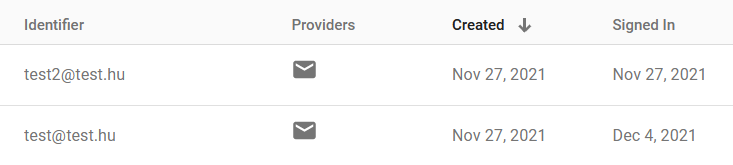
\includegraphics[width=100mm, keepaspectratio]{figures/auth_users.png}
	\caption{A regisztrált felhasználók listája.}
	\label{fig:AuthUsers}
\end{figure}

A bejelentkeztetést a \emph{ui.login} package-ben található \emph{LoginFragment} végzi. Ő a többi képernyővel ellentétben csak egy sima Fragment, nem a RainbowCake architektúra része, ugyanis tulajdonképpen két függvényből áll az egész, így nem tartottam célszerűnek végigvezetni a rétegeken. Ahogy azt a \refstruc{fig:MaterialBeforeAfter} korábban bemutatta, egyetlen képernyő áll rendelkezésre mind a bejelentkezéshez, mind a regisztrációhoz. Ez a döntés azért született meg, mert az alkalmazás jelenlegi funkcionalitásában nincs szerepe a felhasználói profilnak, nincs szükség semmilyen plusz információra a felhasználótól, ami később bármilyen formában felhasználásra kerülne, így felesleges két teljesen ugyanolyan UI-t készíteni csak a megkülönböztetés kedvéért.

Az autentikáció végrehajtásához a Firebase biztosít egy \emph{FirebaseAuth} típusú objektumot, melyen keresztül elérhető az összes ezzel kapcsolatos művelet. Meg lehet nézni, hogy van-e bejelentkezett felhasználó, és ezzel átugorható a bejelentkezési folyamat, ha valaki korábban már használta az alkalmazást. Ha nem, akkor pedig (e-mail és jelszavas bejelentkezés esetén) a \emph{signInWithEmailAndPassword} és a \emph{createUserWithEmailAndPassword} függvények állnak rendelkezésre, melyeknek az e-mail címet és a jelszót paraméterként megadva elvégzik a megfelelő műveletet. Az eredményt aszinkron módon küldi, amire egy \emph{onCompleteListener} segítségével lehet feliratkozni. Ezen belül ellenőrizhető a hívás kimenetele, és sikeres művelet esetén át tudunk navigálni az alkalmazás megfelelő képernyőjére, hiba esetén pedig kezelni tudjuk azt.

A következő szolgáltatás a Firestore, mely adatok felhőalapú tárolását teszi lehetővé egy hierarchikus struktúrában. Bekapcsolása után elérhetővé válik a kezelőfelülete, ahol szabályokat adhatunk meg a hozzáférésre, illetve láthatunk minden tárolt adatot egy könnyen átlátható vizuális reprezentációban. Az alkalmazás adatai az (\refstruc{fig:Firestore}) által mutatott módon kerülnek tárolásra. 

Az összes adat egy \emph{users} nevű kollekcióban található, amiben minden felhasználóhoz tartozik egy dokumentum, melynek neve a regisztrációkor generált UID. Mivel ez garantáltan egyéni, így mindenki csak a saját adatait fogja elérni, és nem fordulhat elő, hogy egy felhasználó tudtán kívül felülírja egy másik adatait. A felhasználók dokumentumai két kollekciót tárolnak: egyet a kategóriáknak, és egyet a jegyzeteknek. Ezeken belül egy-egy dokumentum tárol egy-egy jegyzetet illetve kategóriát, melyeknek szintén egyéni azonosítója van. 

Az alkalmazásban a \emph{data.network} package-ben található \emph{FirebaseApi} nevű osztály végzi az adatok lekérését és objektumokká való konvertálását. Az adatbázist egy \emph{FirebaseFirestore} típusú objektumon keresztül érem el, a \refstruc{fig:FirestoreQuery} által mutatott kóddal. 

\begin{figure}[!ht]
	\centering
	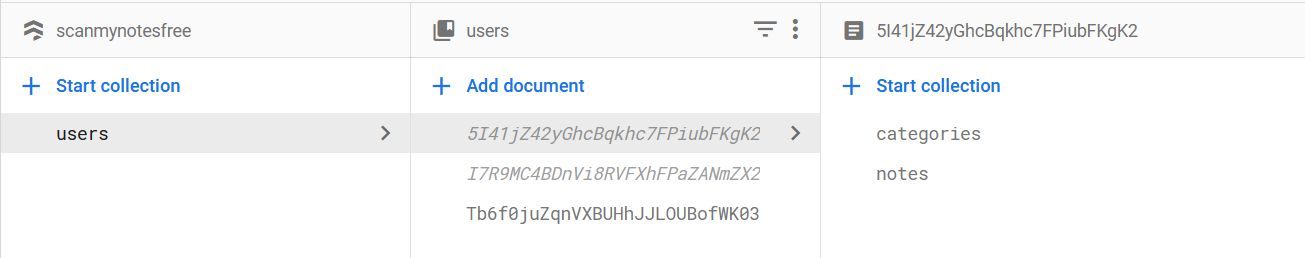
\includegraphics[width=150mm, keepaspectratio]{figures/firestore.png}
	\caption{A felhasználók adatainak struktúrája.}
	\label{fig:Firestore}
\end{figure}

\begin{figure}[!ht]
	\centering
	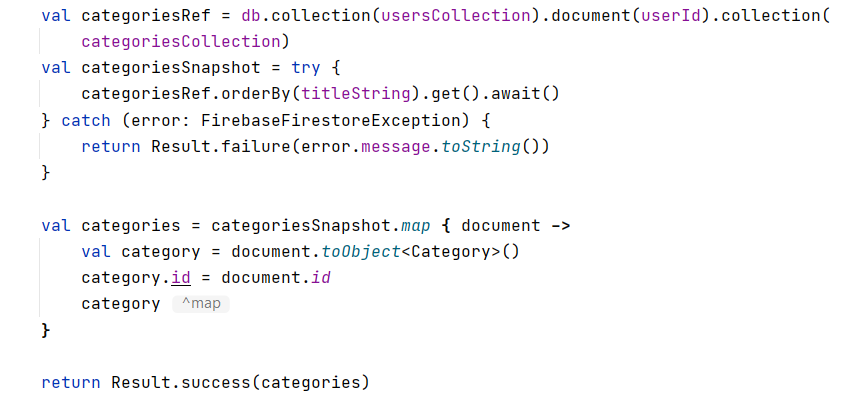
\includegraphics[width=150mm, keepaspectratio]{figures/firestore_query.png}
	\caption{A kategóriák lekérésének kódja az adatbázisból.}
	\label{fig:FirestoreQuery}
\end{figure}

Itt a \emph{db} változó az a bizonyos objektum, melyen keresztül elérhető az adatbázis. A hívástól függően egy \emph{CollectionReference} vagy egy \emph{DocumentReference} lehet az eredmény, ami az adott kollekció/dokumentum helyére mutat. Ezek felhasználhatók adatok írására és olvasására, ha pedig nem létezik adat azon a helyen, akkor létrehozza azt. Alapértelmezetten a referenciákon végzett minden hívás aszinkron módon hajtódik végre, de ez a működés nem volt ideális az alkalmazásom számára, ezért a \emph{kotlinx.coroutines.tasks.await()} függvény segítségével bevárom a lekérdezés eredményét. Ezután már csak annyi van hátra, hogy a visszakapott Snapshot objektumból kialakítsam azokat a típusokat, amikre szüksége van az alkalmazásnak. Szerencsére ez rendkívül egyszerű, mivel a Firestore biztosít egy \emph{toObject} függvényt, melynek a kívánt típust template-paraméterként megadva elvégzi a konverziót. Az id-t pedig azért kell még utána beállítani a kapott objektumon, mert az nem egy tárolt mezője a dokumentumnak, hanem az azonosítója, így arra nem terjed ki a \emph{toObject}.

A harmadik szolgáltatás az Analytics, mely rengeteg hasznos információt szolgáltat a felhasználókról és szokásaikról. Az előzőekhez hasonlóan itt is egy objektum biztosítja a kívánt funkcionalitást, melynek típusa ez esetben \emph{FirebaseAnalytics}. Ez figyel pár darab beépített eseményt, mint például a képernyők látogatását vagy a munkamenet-kezdést, de sajátot is lehet definiálni (\refstruc{fig:Analytics}). Itt egy új felhasználó regisztrációját rögzíti a rendszer annak metódusával együtt, ami jelen esetben e-mail és jelszó. 

\begin{figure}[!ht]
	\centering
	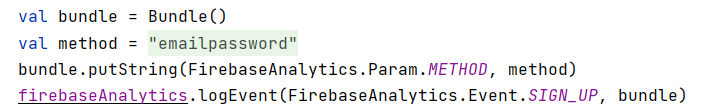
\includegraphics[width=120mm, keepaspectratio]{figures/analytics_custom.png}
	\caption{Egyéni esemény létrehozása és logolása Analytics segítségével.}
	\label{fig:Analytics}
\end{figure}

Az utolsó Firebase szolgáltatás, amit az alkalmazásban felhasználtam, a Crashlytics. Az előzőektől ellentétben az első bekezdésben leírtakon kívül ennél még szükség van további integrációs lépésekre is a működéshez. Van ugyanis egy saját pluginja, amit a fentiekkel megegyező módon fel kell venni mindkét gradle fájlba. Ezt követően szükség van egy teszt crash előidézésére, majd az alkalmazás újraindítására, hogy az elküldhesse a hibajelentést a Crashlyticsnek. Ezt követően viszont nincs már szükség semmi másra, a kódba sem szükséges semmit felvenni, mert automatikusan figyeli az alkalmazást. Természetesen számos lehetőségünk van finomhangolni a működését egyéni kulcsok hozzáadásával, de akár a nem-végzetes hibák figyelésével is.

\subsection{Képfelismerés integrációja}

\subsection{Modellek elkészítése} 

\subsection{Összetett lista}

\subsection{Navigáció}

\section{Működés}

A következőkben az alkalmazás funkcióit fogom bemutatni, a leírásokat képernyőképekkel kiegészítve. A képek néhol eltérnek egymástól, melynek oka hogy az applikáció funkcionalitásából fakadóan nem volt lehetséges mindet az emulátoron elkészíteni, hanem a jegyzetek készítéséhez fizikai készülékre is szükség volt.

\subsection{Bejelentkezés}
A telepítést követően a bejelentkezési képernyő az első, amivel a felhasználó találkozik. Ez már korábban megjelent a dolgozatban, a \refstruc{fig:MaterialBeforeAfter} bemutatásában. Itt a beviteli mezők segédszövegei egyértelműsítik, hogy milyen adatok elvártak a bejelentkezéshez illetve regisztrációhoz. Ezek gombnyomás hatására validálásra kerülnek, és amennyiben az e-mail formátuma nem érvényes vagy a jelszó hossza nem éri el a 6 karaktert, akkor a folyamat meghiúsul, és a felhasználó értesül róla, hogy mely mező(k) tartalmát kell javítania. 
%TODO picture if short on pages

\subsection{Kategorizált lista}
Sikeres bejelentkezést követően az alkalmazás a fő képernyőjére navigál, ahol az eddig elmentett jegyzeteket láthatjuk kategóriákba rendezve. A kategóriák alapértelmezetten össze vannak csukva, csak a legfelső szinten található elemeket látjuk. A lista sorainak jobb szélén elhelyezkedő nyilakra kattintva tudjuk kibontani az adott kategóriát, ezzel megtekinteni a tartalmát (\refstruc{fig:NoteListScreen}).

\begin{figure}[!ht]
	\centering
	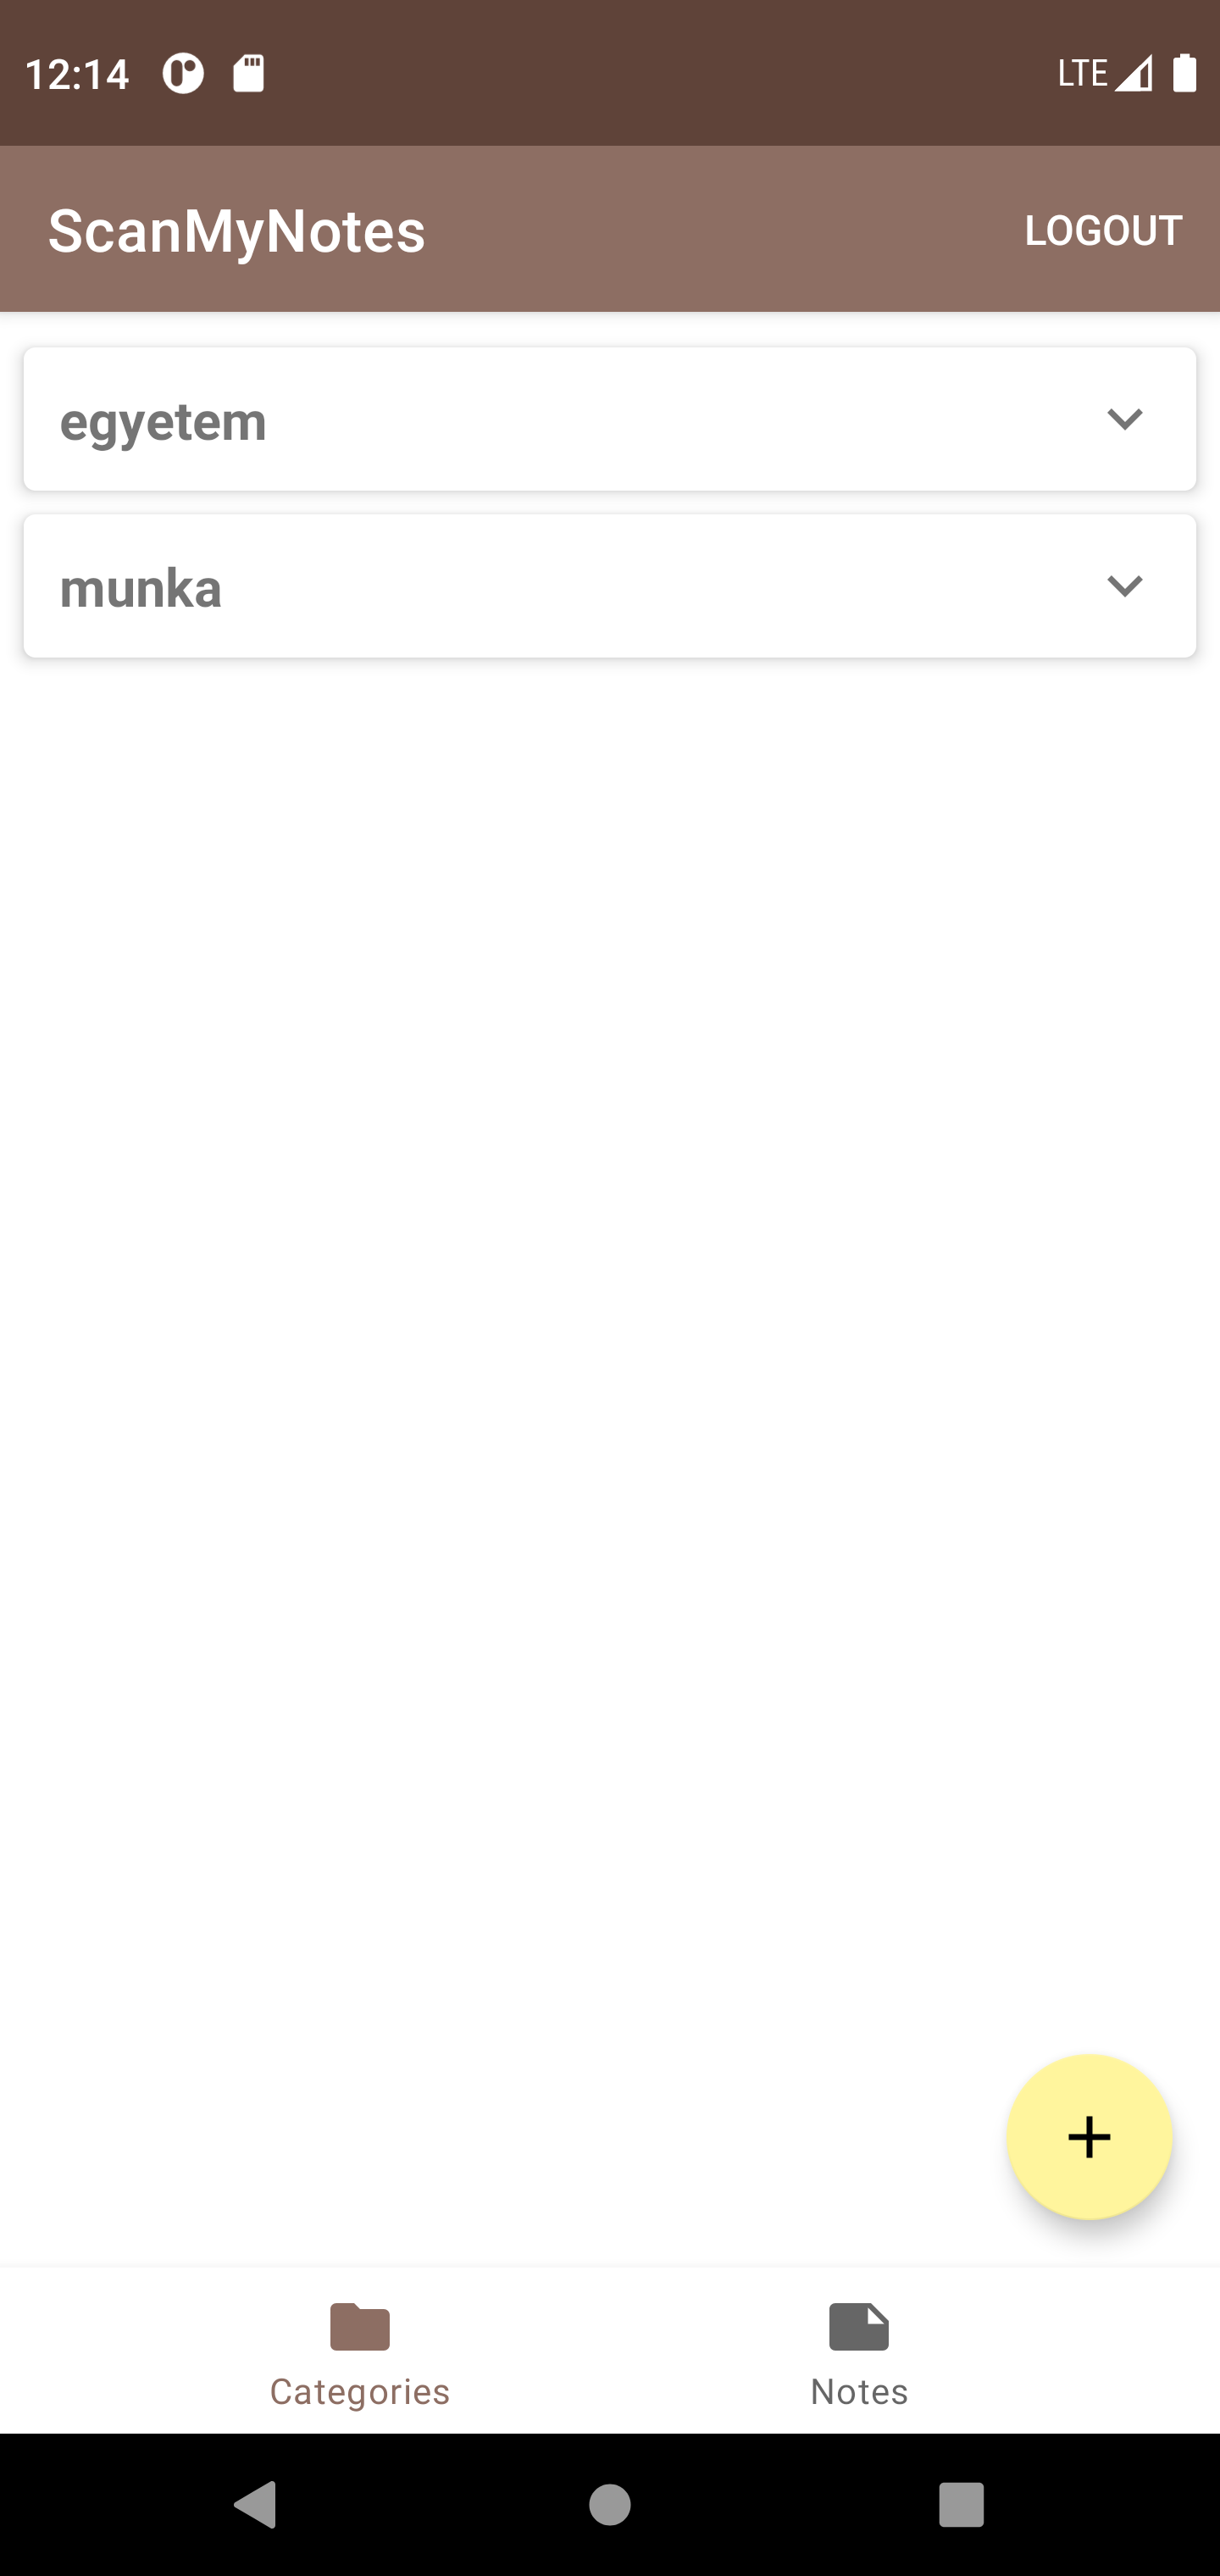
\includegraphics[width=55mm, keepaspectratio]{figures/notelist_closed.png}
	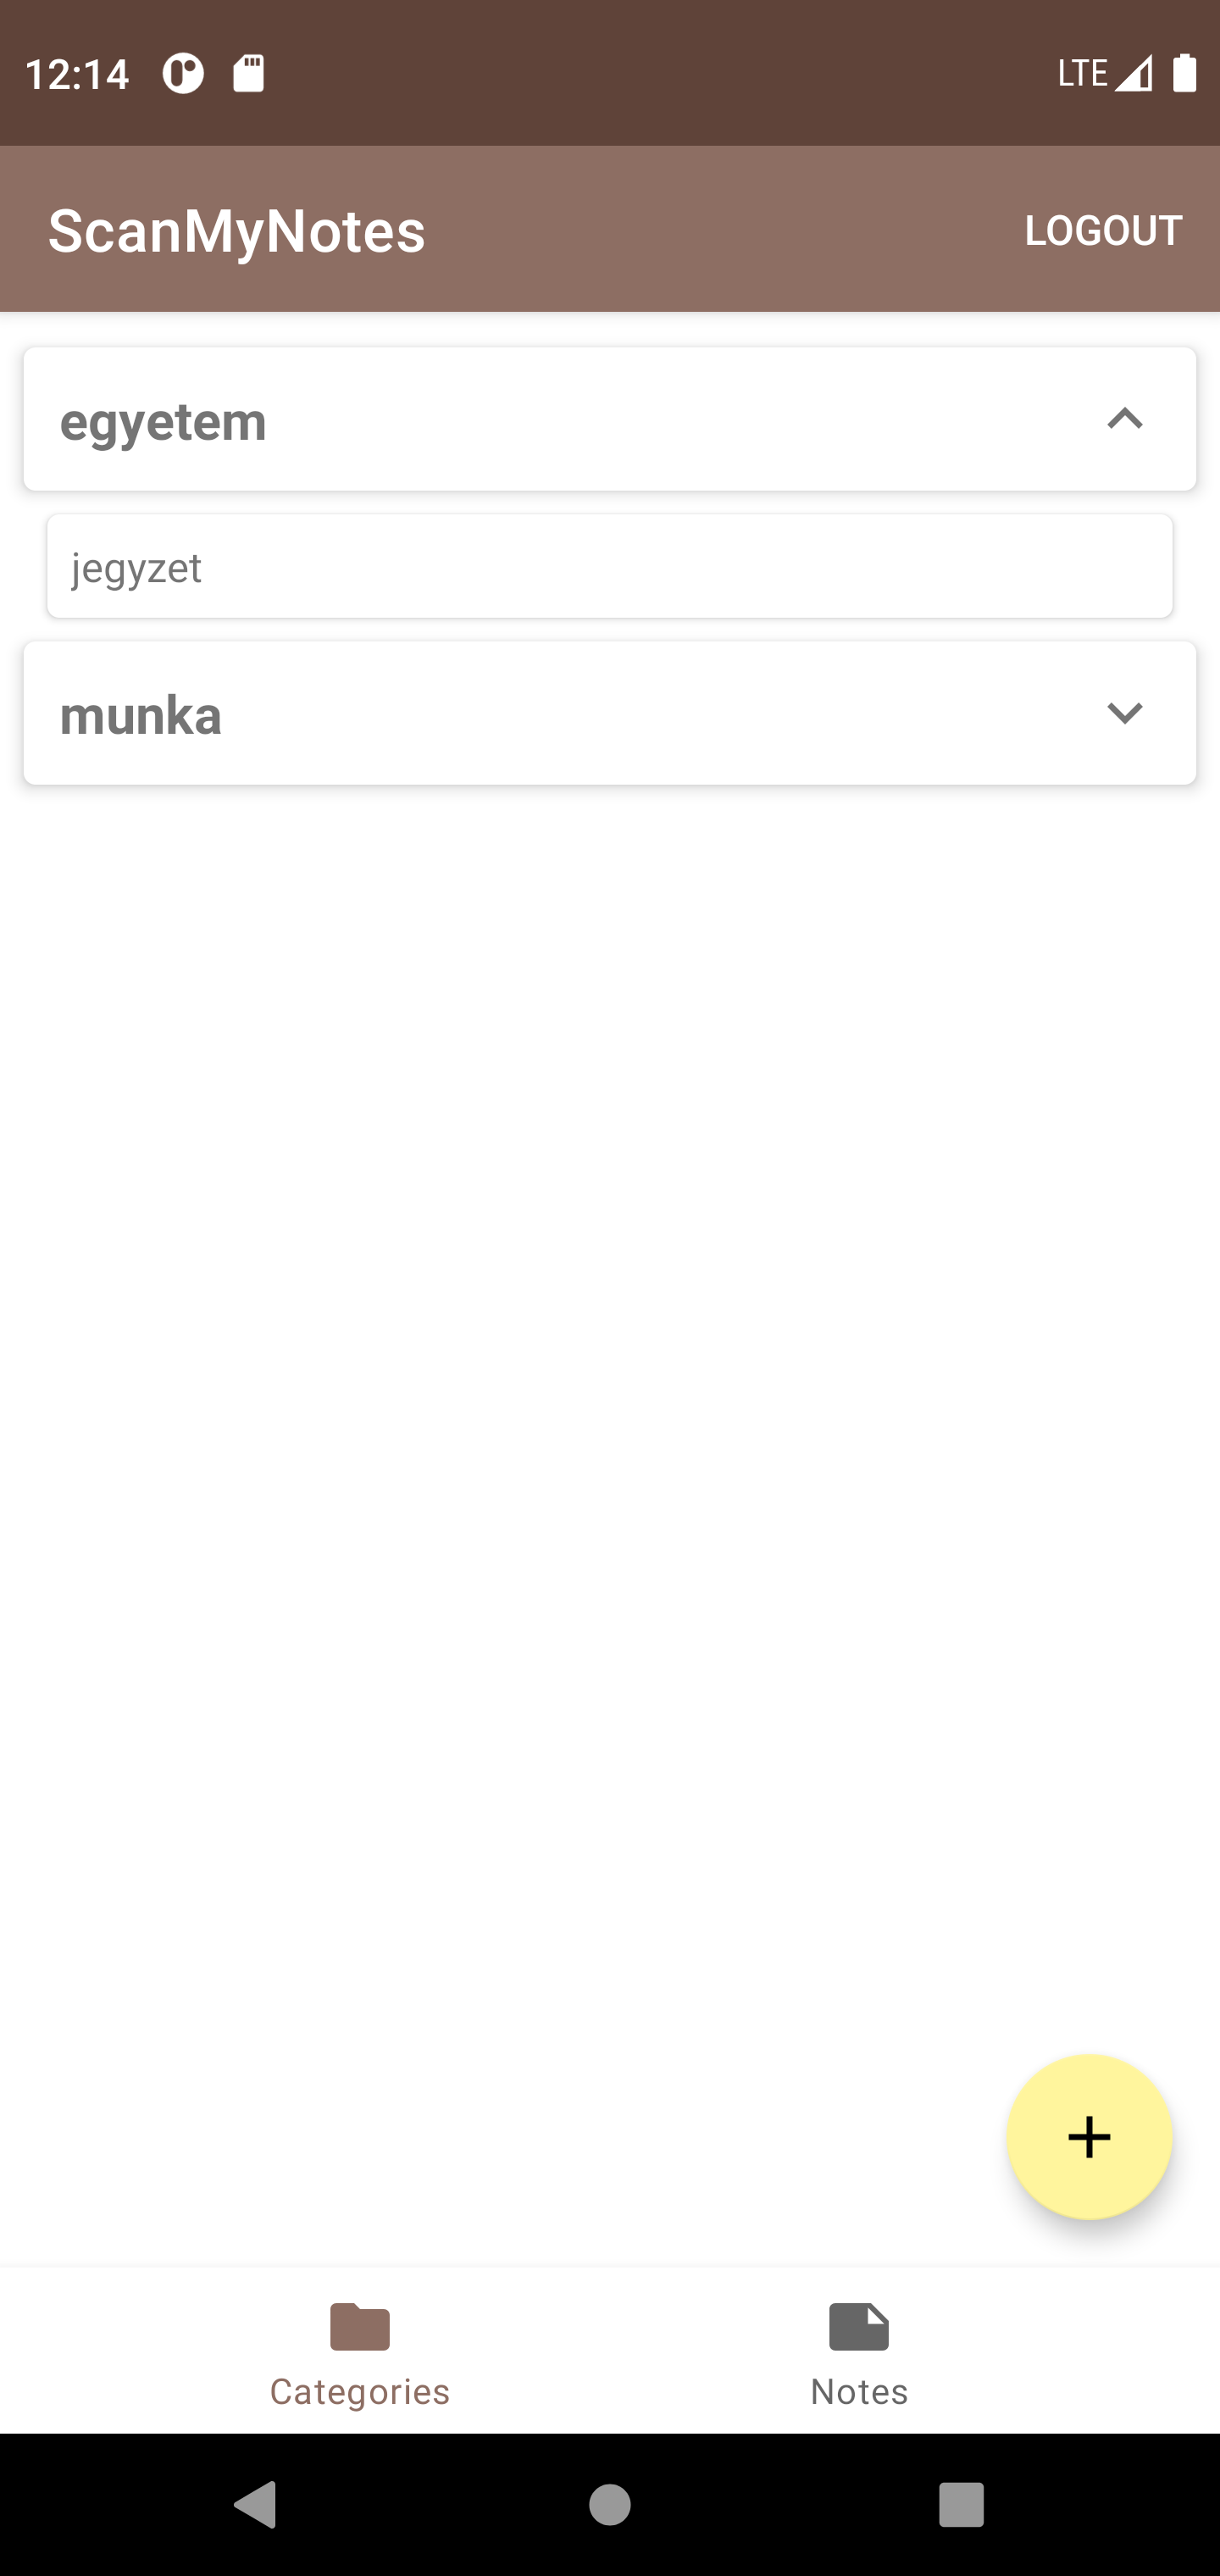
\includegraphics[width=55mm, keepaspectratio]{figures/notelist_open.png}
	\caption{Az alkalmazás kezdőlapja alapértelmezett állapotban, illetve egy kategória kibontva.}
	\label{fig:NoteListScreen}
\end{figure}

Innen számos lehetőségünk adódik navigációra az applikáción belül, kezdve a jobb felső sarokban található, meglehetősen magától értetődő kijelentkezés gombbal. Ezt megnyomva a fent leírt bejelentkezési képernyőre navigálunk, ahol adataink megadásával újra bejelentkezhetünk.

\subsection{Jegyzetlista}
A főképernyőn alul egy navigációs sávot találunk, mellyel a két különböző listamegjelenítés között tudunk váltani. Míg a \emph{Categories} opció alatt egy hierarchikusan egymás alá rendezett listát láthatunk, a \emph{Notes} opció csak a jegyzeteket tárja elénk, kategóriától függetlenül. Itt több lehetőség tárul elénk: a képernyő tetején található egy keresősáv és egy rendezés gomb. Keresni a jegyzetek címe alapján tudunk, itt gépelés közben azonnal szűkül az eredményhalmaz. A rendezés szintén a cím alapján működik, jelenleg növekvő és csökkenő betűrendet támogat az alkalmazás (\refstruc{fig:NoteListScreen2}). 

\begin{figure}[!ht]
	\centering
	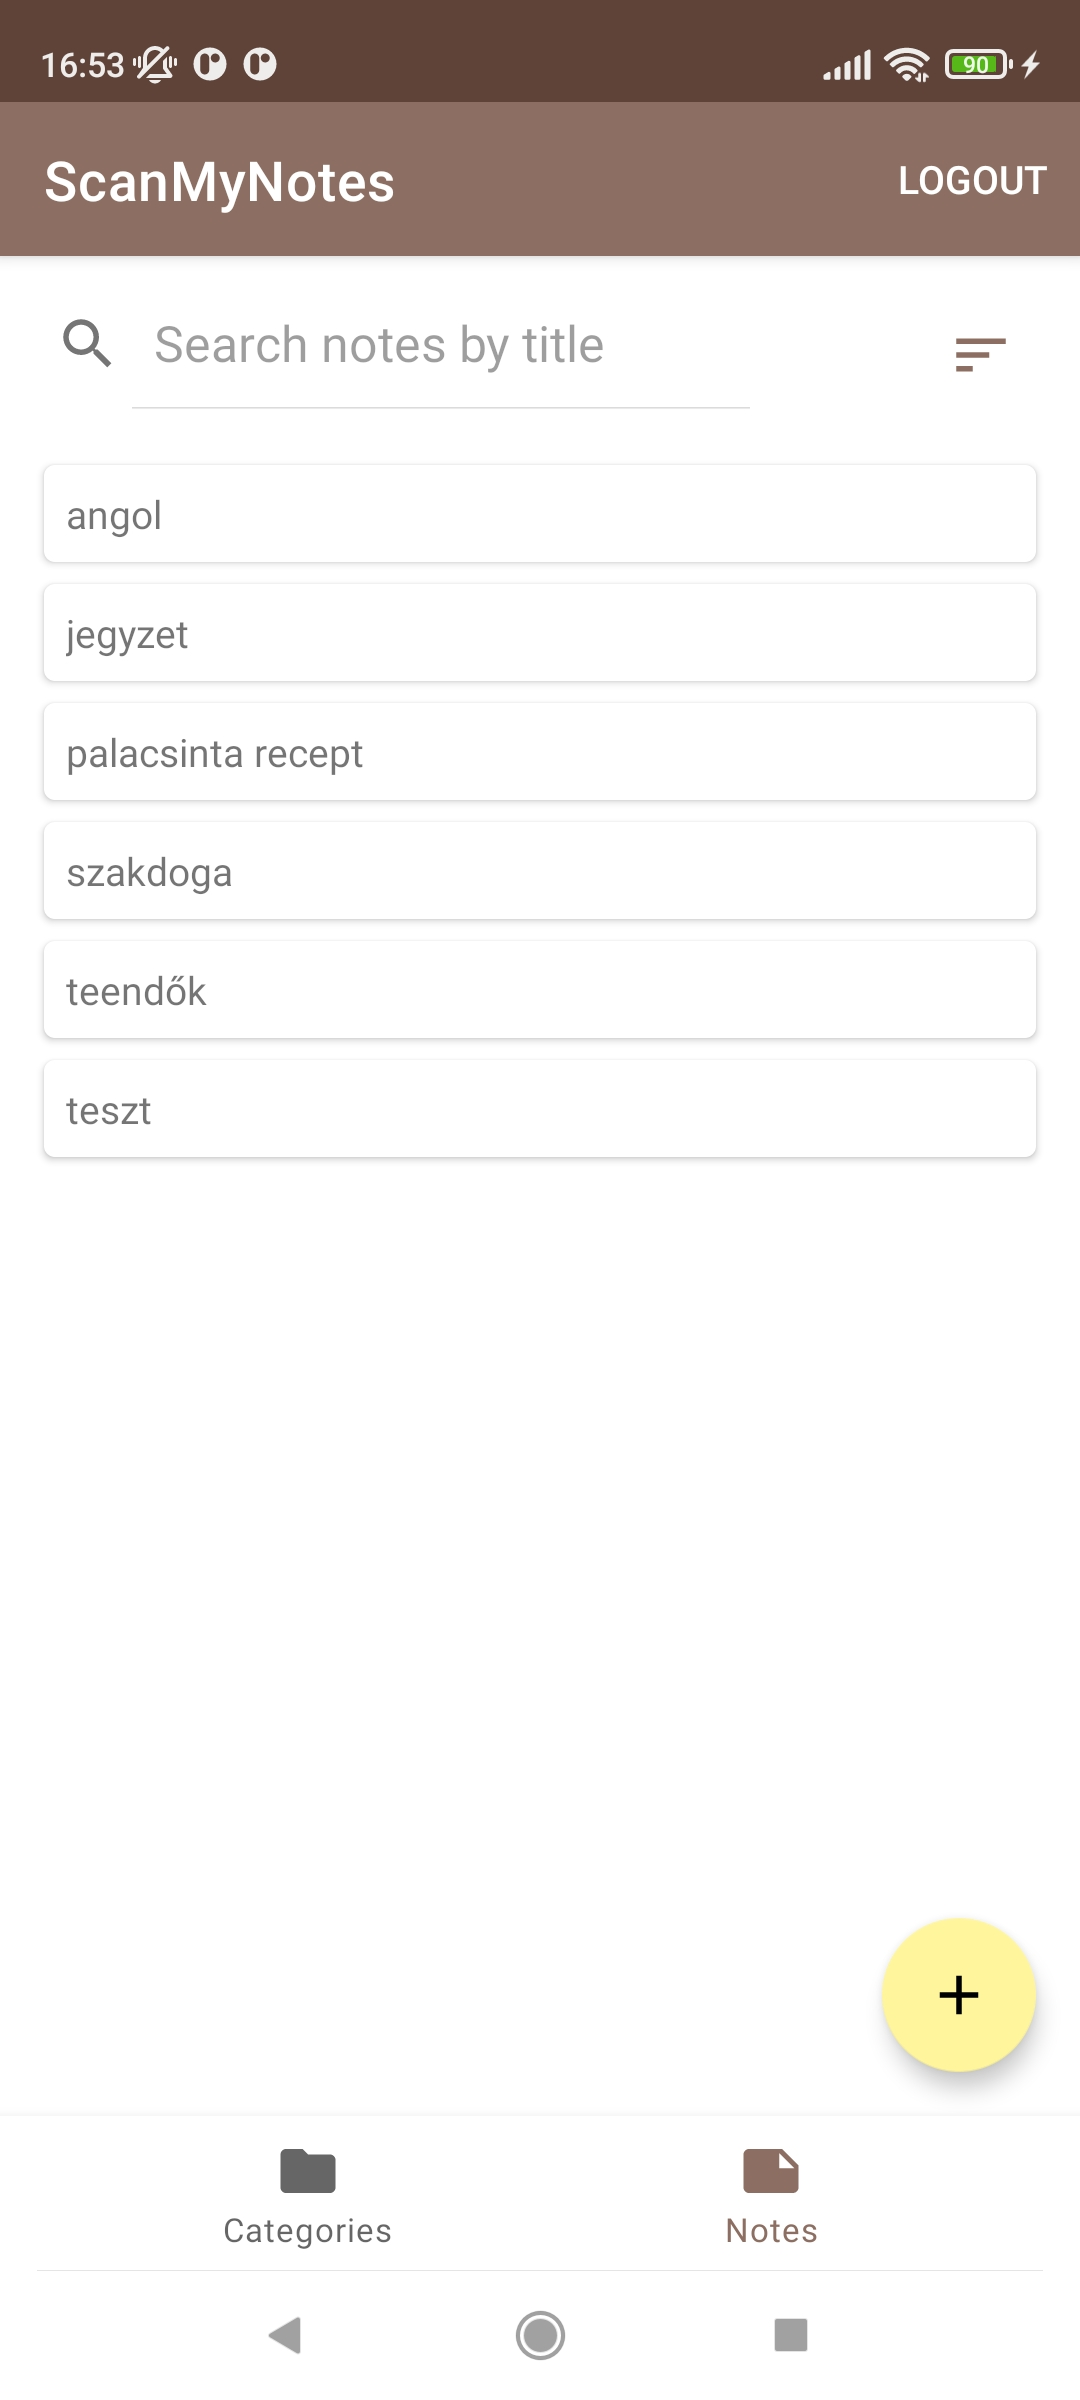
\includegraphics[width=49mm, keepaspectratio]{figures/notelist_full.jpg}
	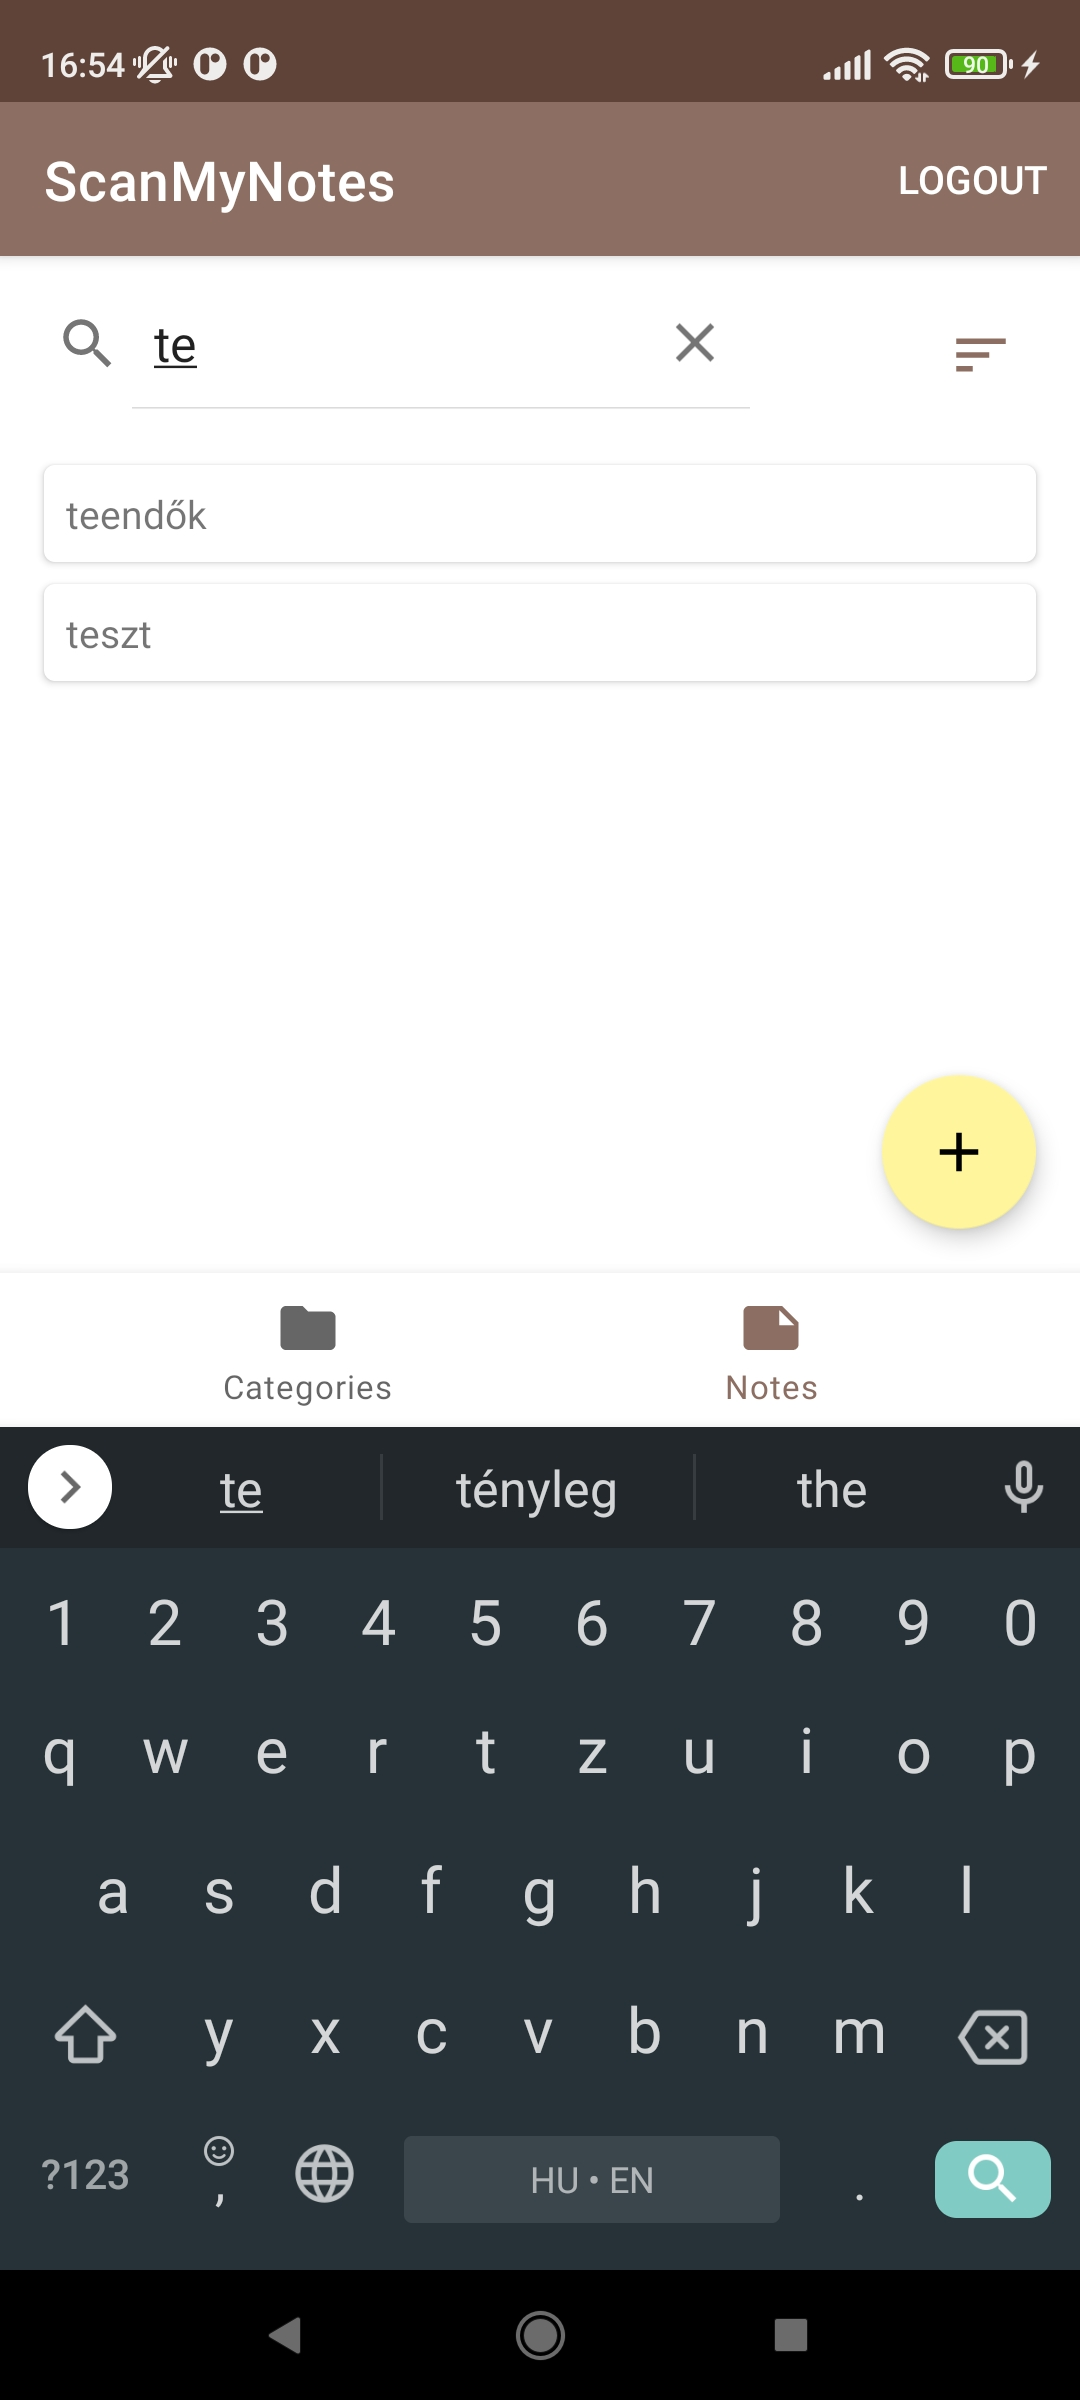
\includegraphics[width=49mm, keepaspectratio]{figures/notelist_search.jpg}
	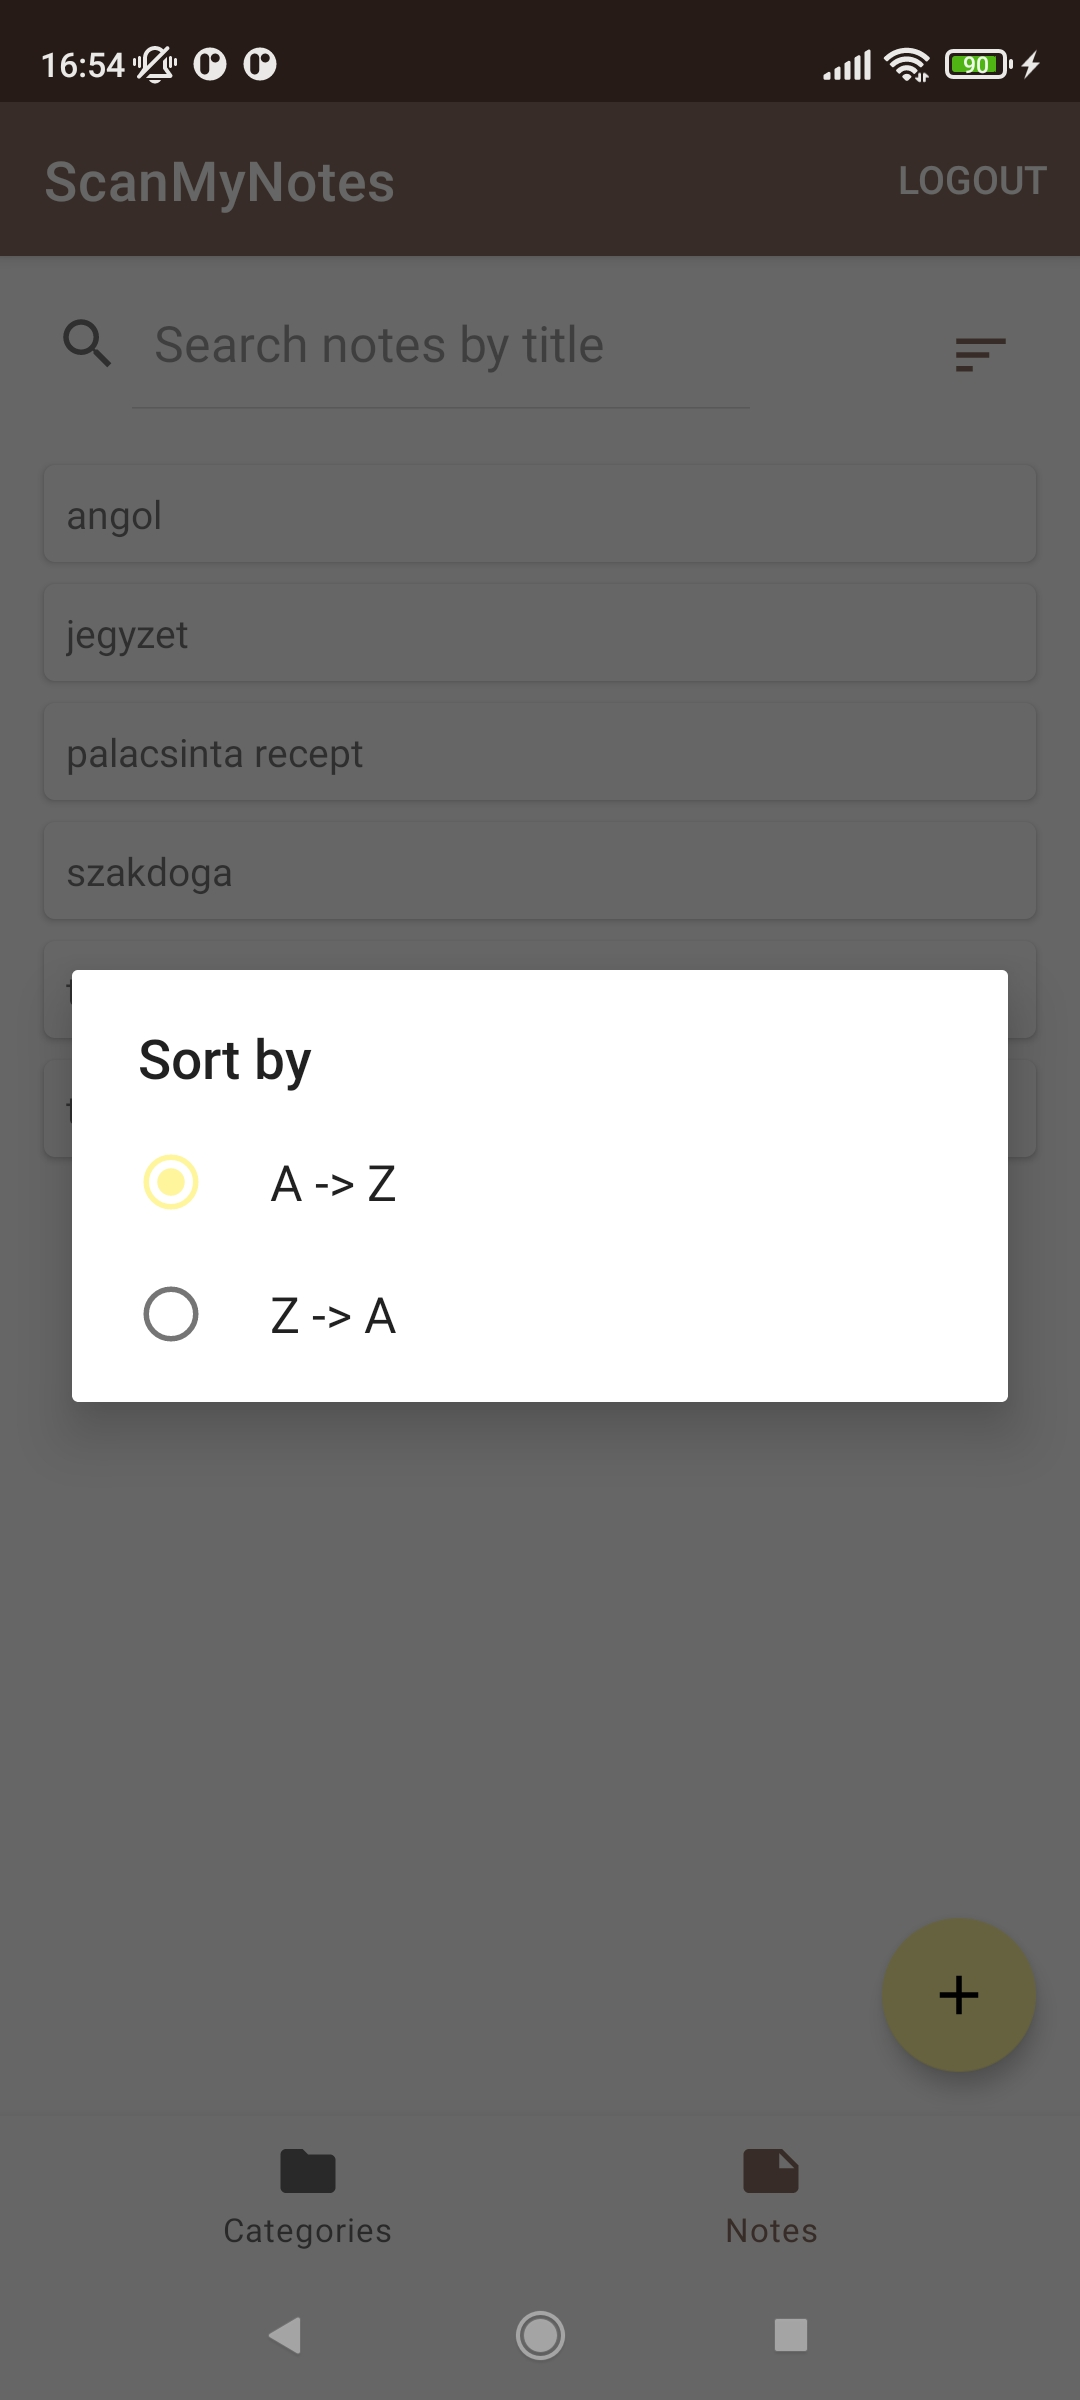
\includegraphics[width=49mm, keepaspectratio]{figures/notelist_sort.jpg}
	\caption{A jegyzetek listája, és a rajta elvégezhető műveletek.}
	\label{fig:NoteListScreen2}
\end{figure}

\subsection{Jegyzet létrehozása}
Az alkalmazás fő funkcionalitása a jegyzetek tárolása, így elég fontos, hogy legyen lehetőség újak létrehozására. Ez a képernyő jobb alsó sarkában található plusz gombra kattintva tehető meg. Az ott megjelenő két újabb gomb közül az alsó megnyomására felugrik egy kameraablak, ahol egy fénykép készítése után megtörténik a digitalizáció, és a szerkesztési oldalra ugrunk. Itt egy cím megadásával fejezhetjük be a létrehozási folyamatot, de opcionálisan hozzárendelhetjük egy kategóriához is (\refstruc{fig:NewNoteScreen}). Amíg a cím vagy a tartalom üres, addig az alkalmazás nem fogja engedni elmenteni a jegyzetet, figyelmeztetést rak az üresen hagyott mezőre.
\begin{figure}[!ht]
	\centering
	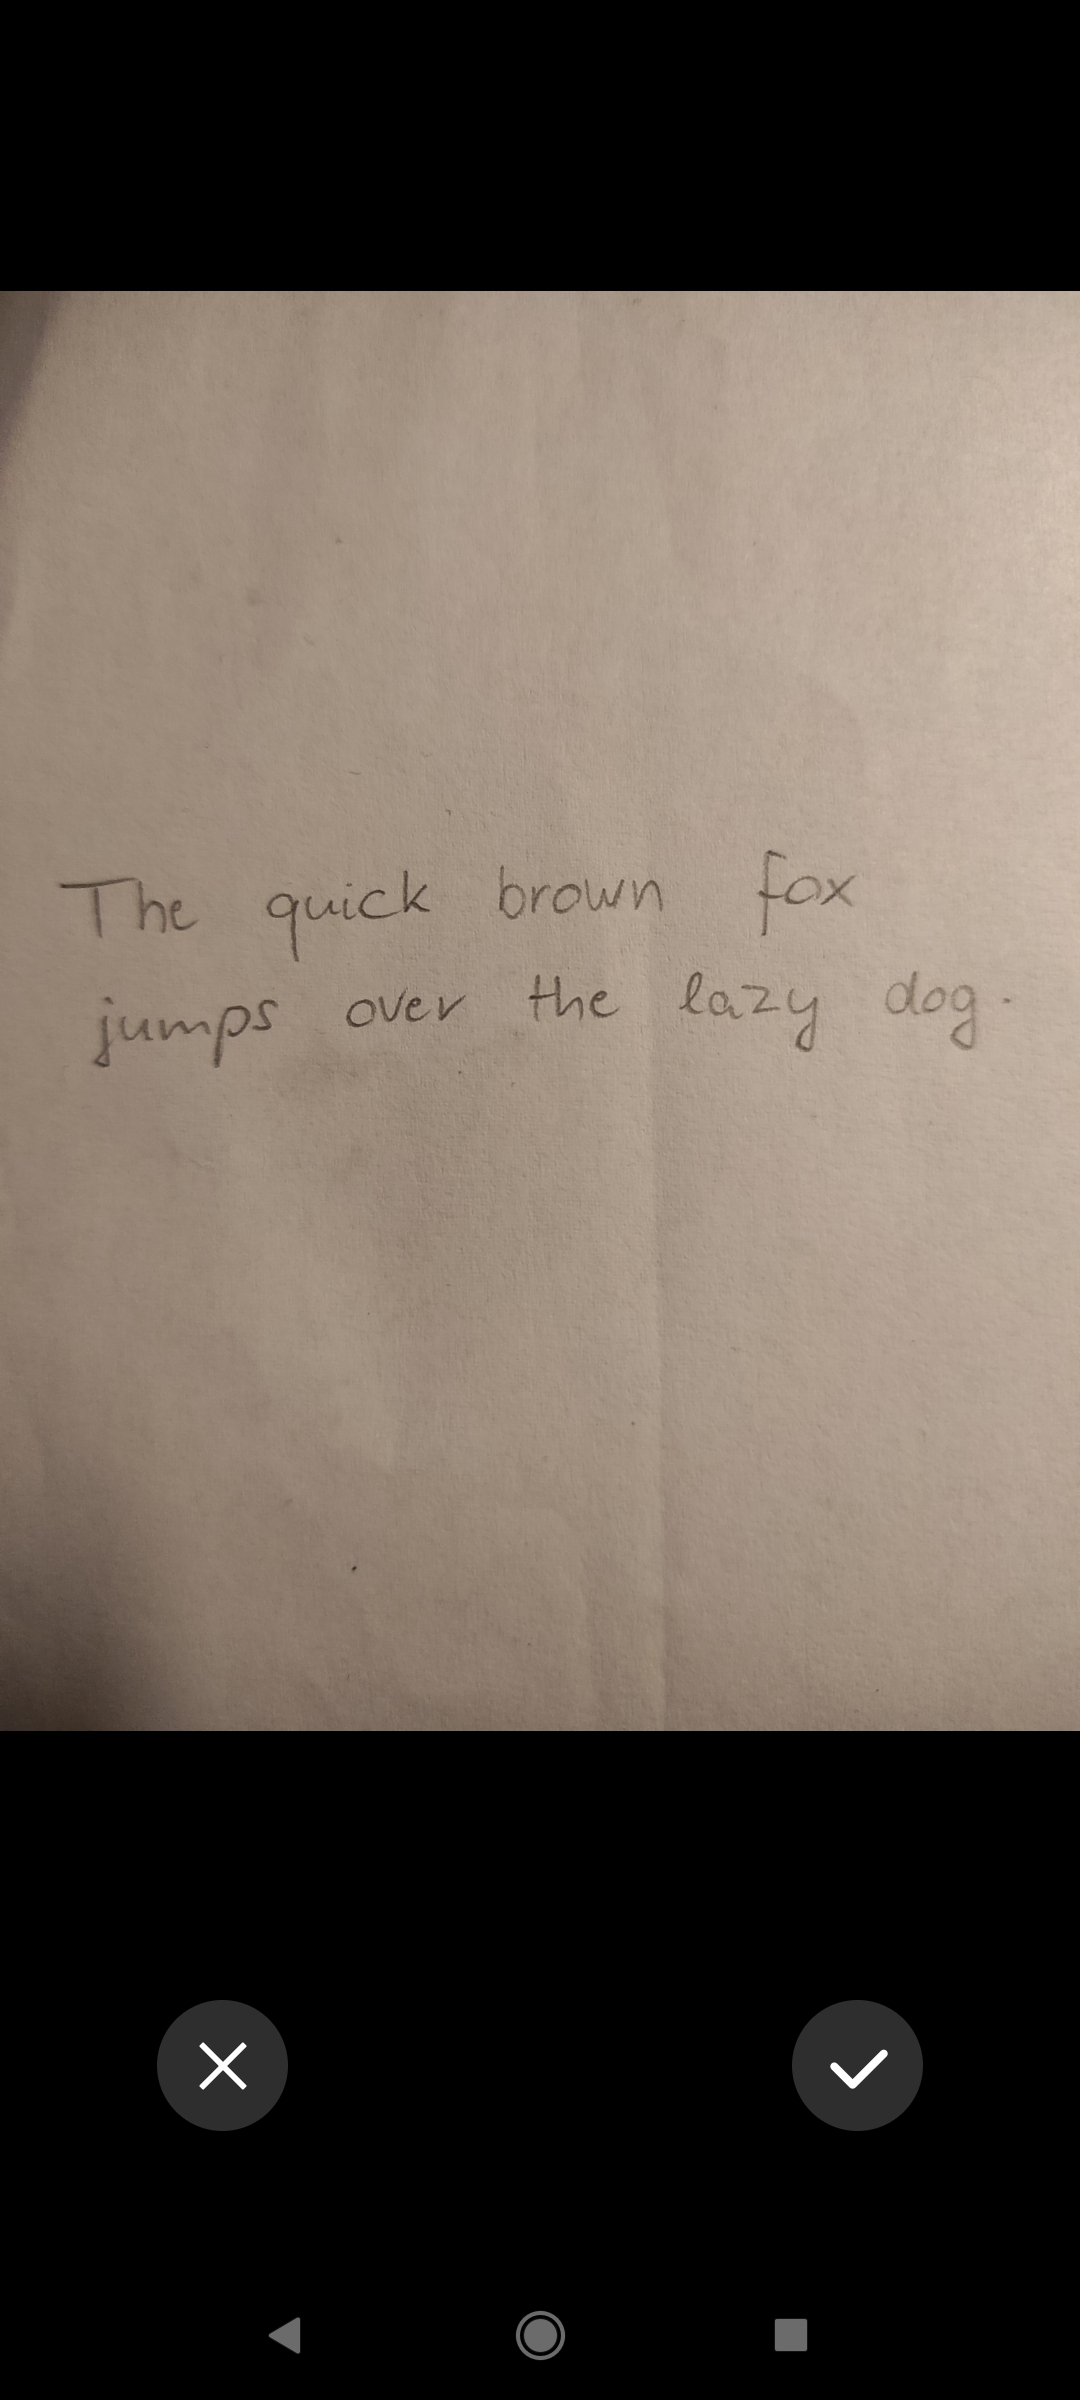
\includegraphics[width=55mm, keepaspectratio]{figures/newnote_photo.jpg}
	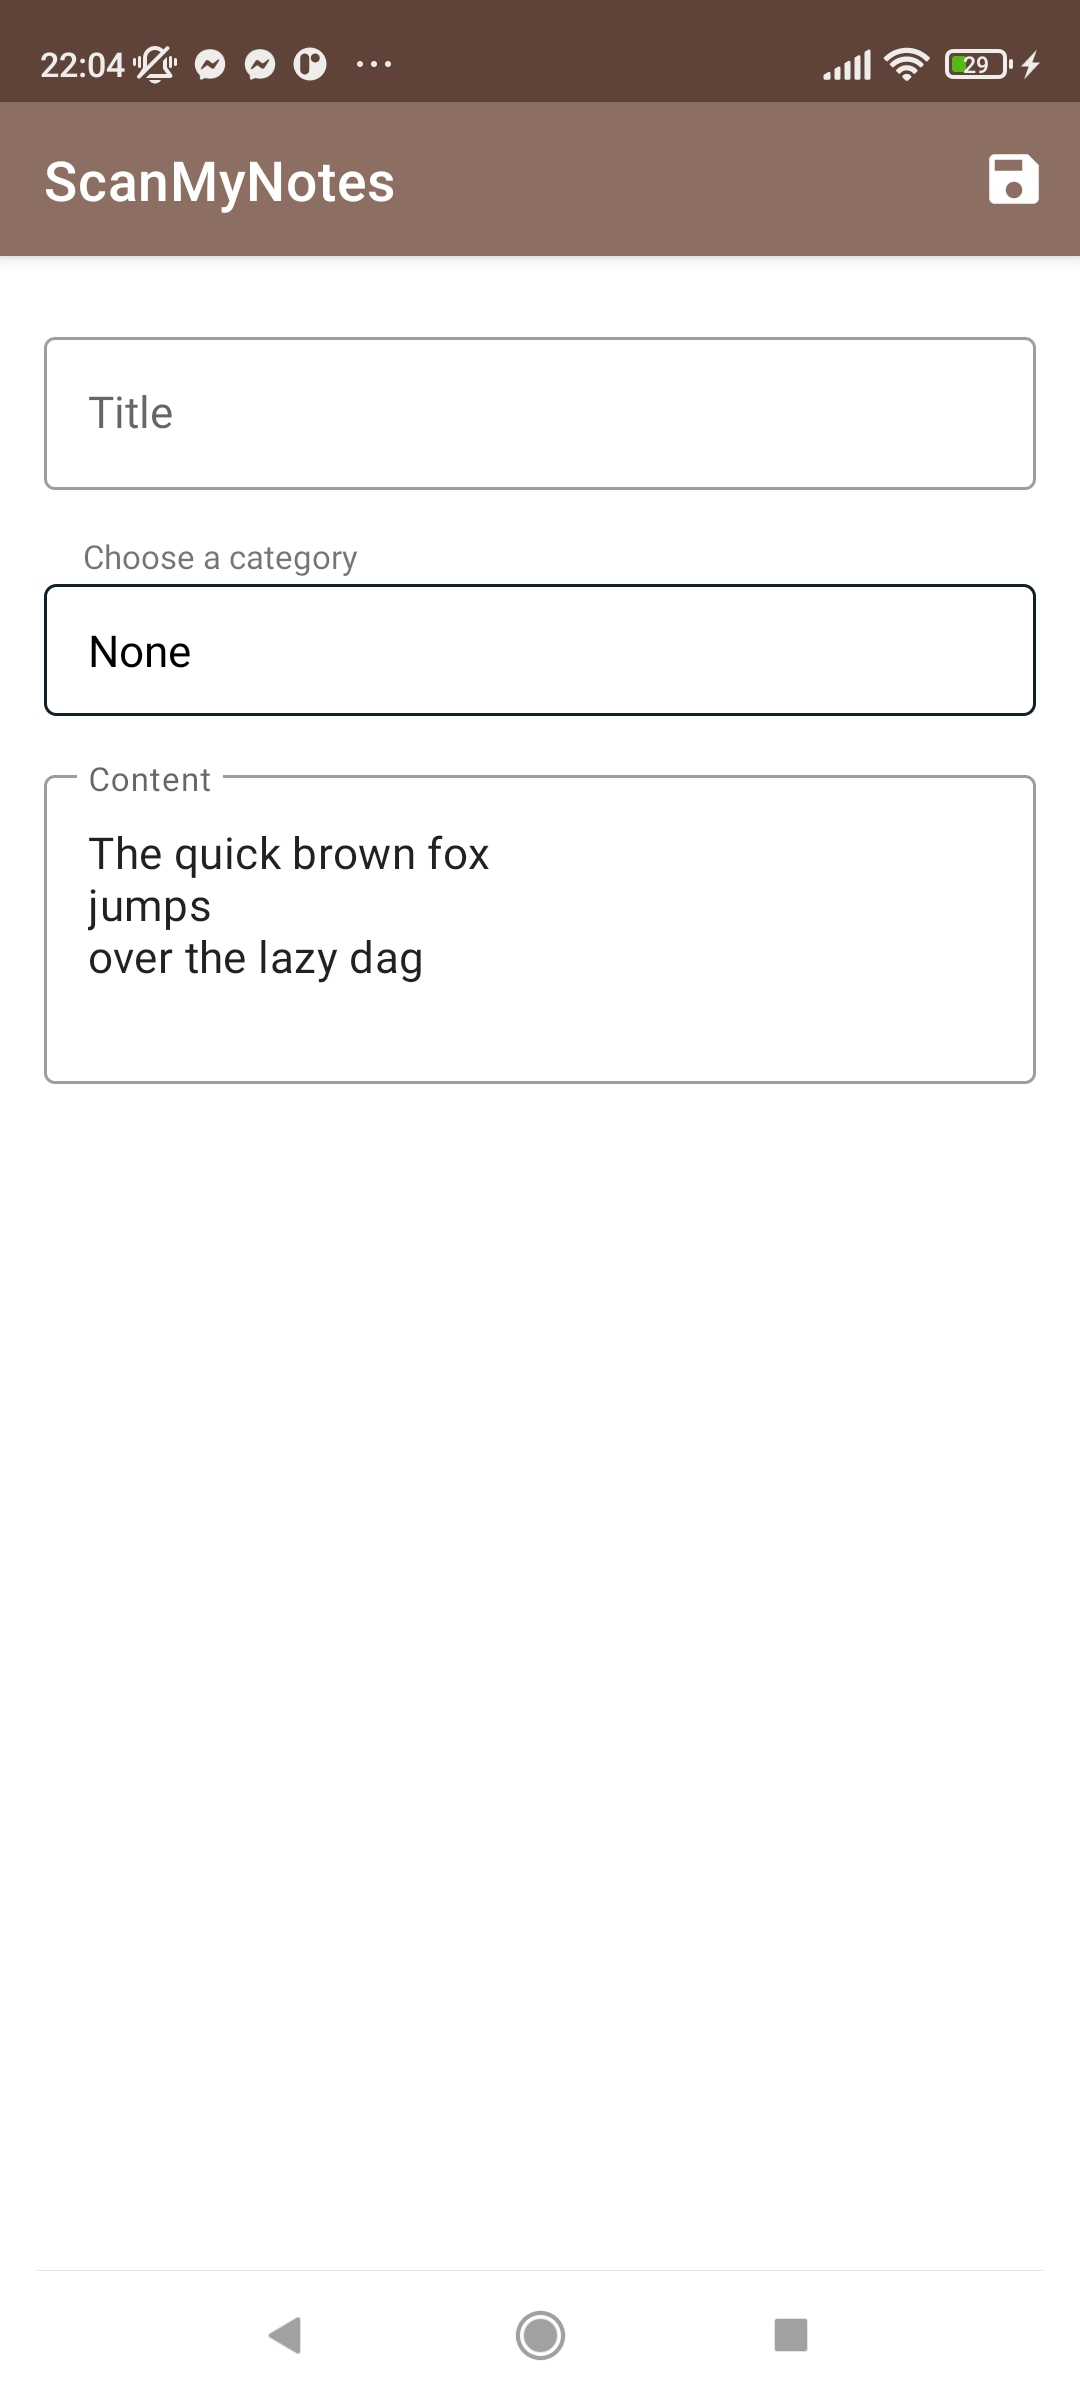
\includegraphics[width=55mm, keepaspectratio]{figures/newnote_create.jpg}
	\caption{A létrehozás során készített kép, illetve az abból kialakuló jegyzet szerkesztése.}
	\label{fig:NewNoteScreen}
\end{figure}

\subsection{Jegyzet szerkesztése}
Amennyiben a listában egy jegyzetre kattintunk, illetve újat hozunk létre, akkor annak részletes oldalára navigálunk. Itt megtekinthetjük a tartalmát, a jobb felső sarokban található ceruza ikonra nyomva pedig szerkeszthetjük is (\refstruc{fig:NoteDetailsScreen}). Megváltoztathatjuk a címét, tartalmát, kategóriáját, a fent megjelenő pluszjel segítségével pedig készíthetünk újabb fotót, melynek szövege hozzáfűzésre kerül az eddigihez. A fentebb említett megkötések itt is érvényesek, azaz a cím és a tartalom nem lehet üres az elmentés pillanatában. 

Mind megtekintési, mind szerkesztési módban elérhető a fenti sávban a szemetes ikon, mellyel törölhetjük a jegyzetet a listánkból. Vigyázat, ez a művelet nem visszafordítható! 

\begin{figure}[!ht]
	\centering
	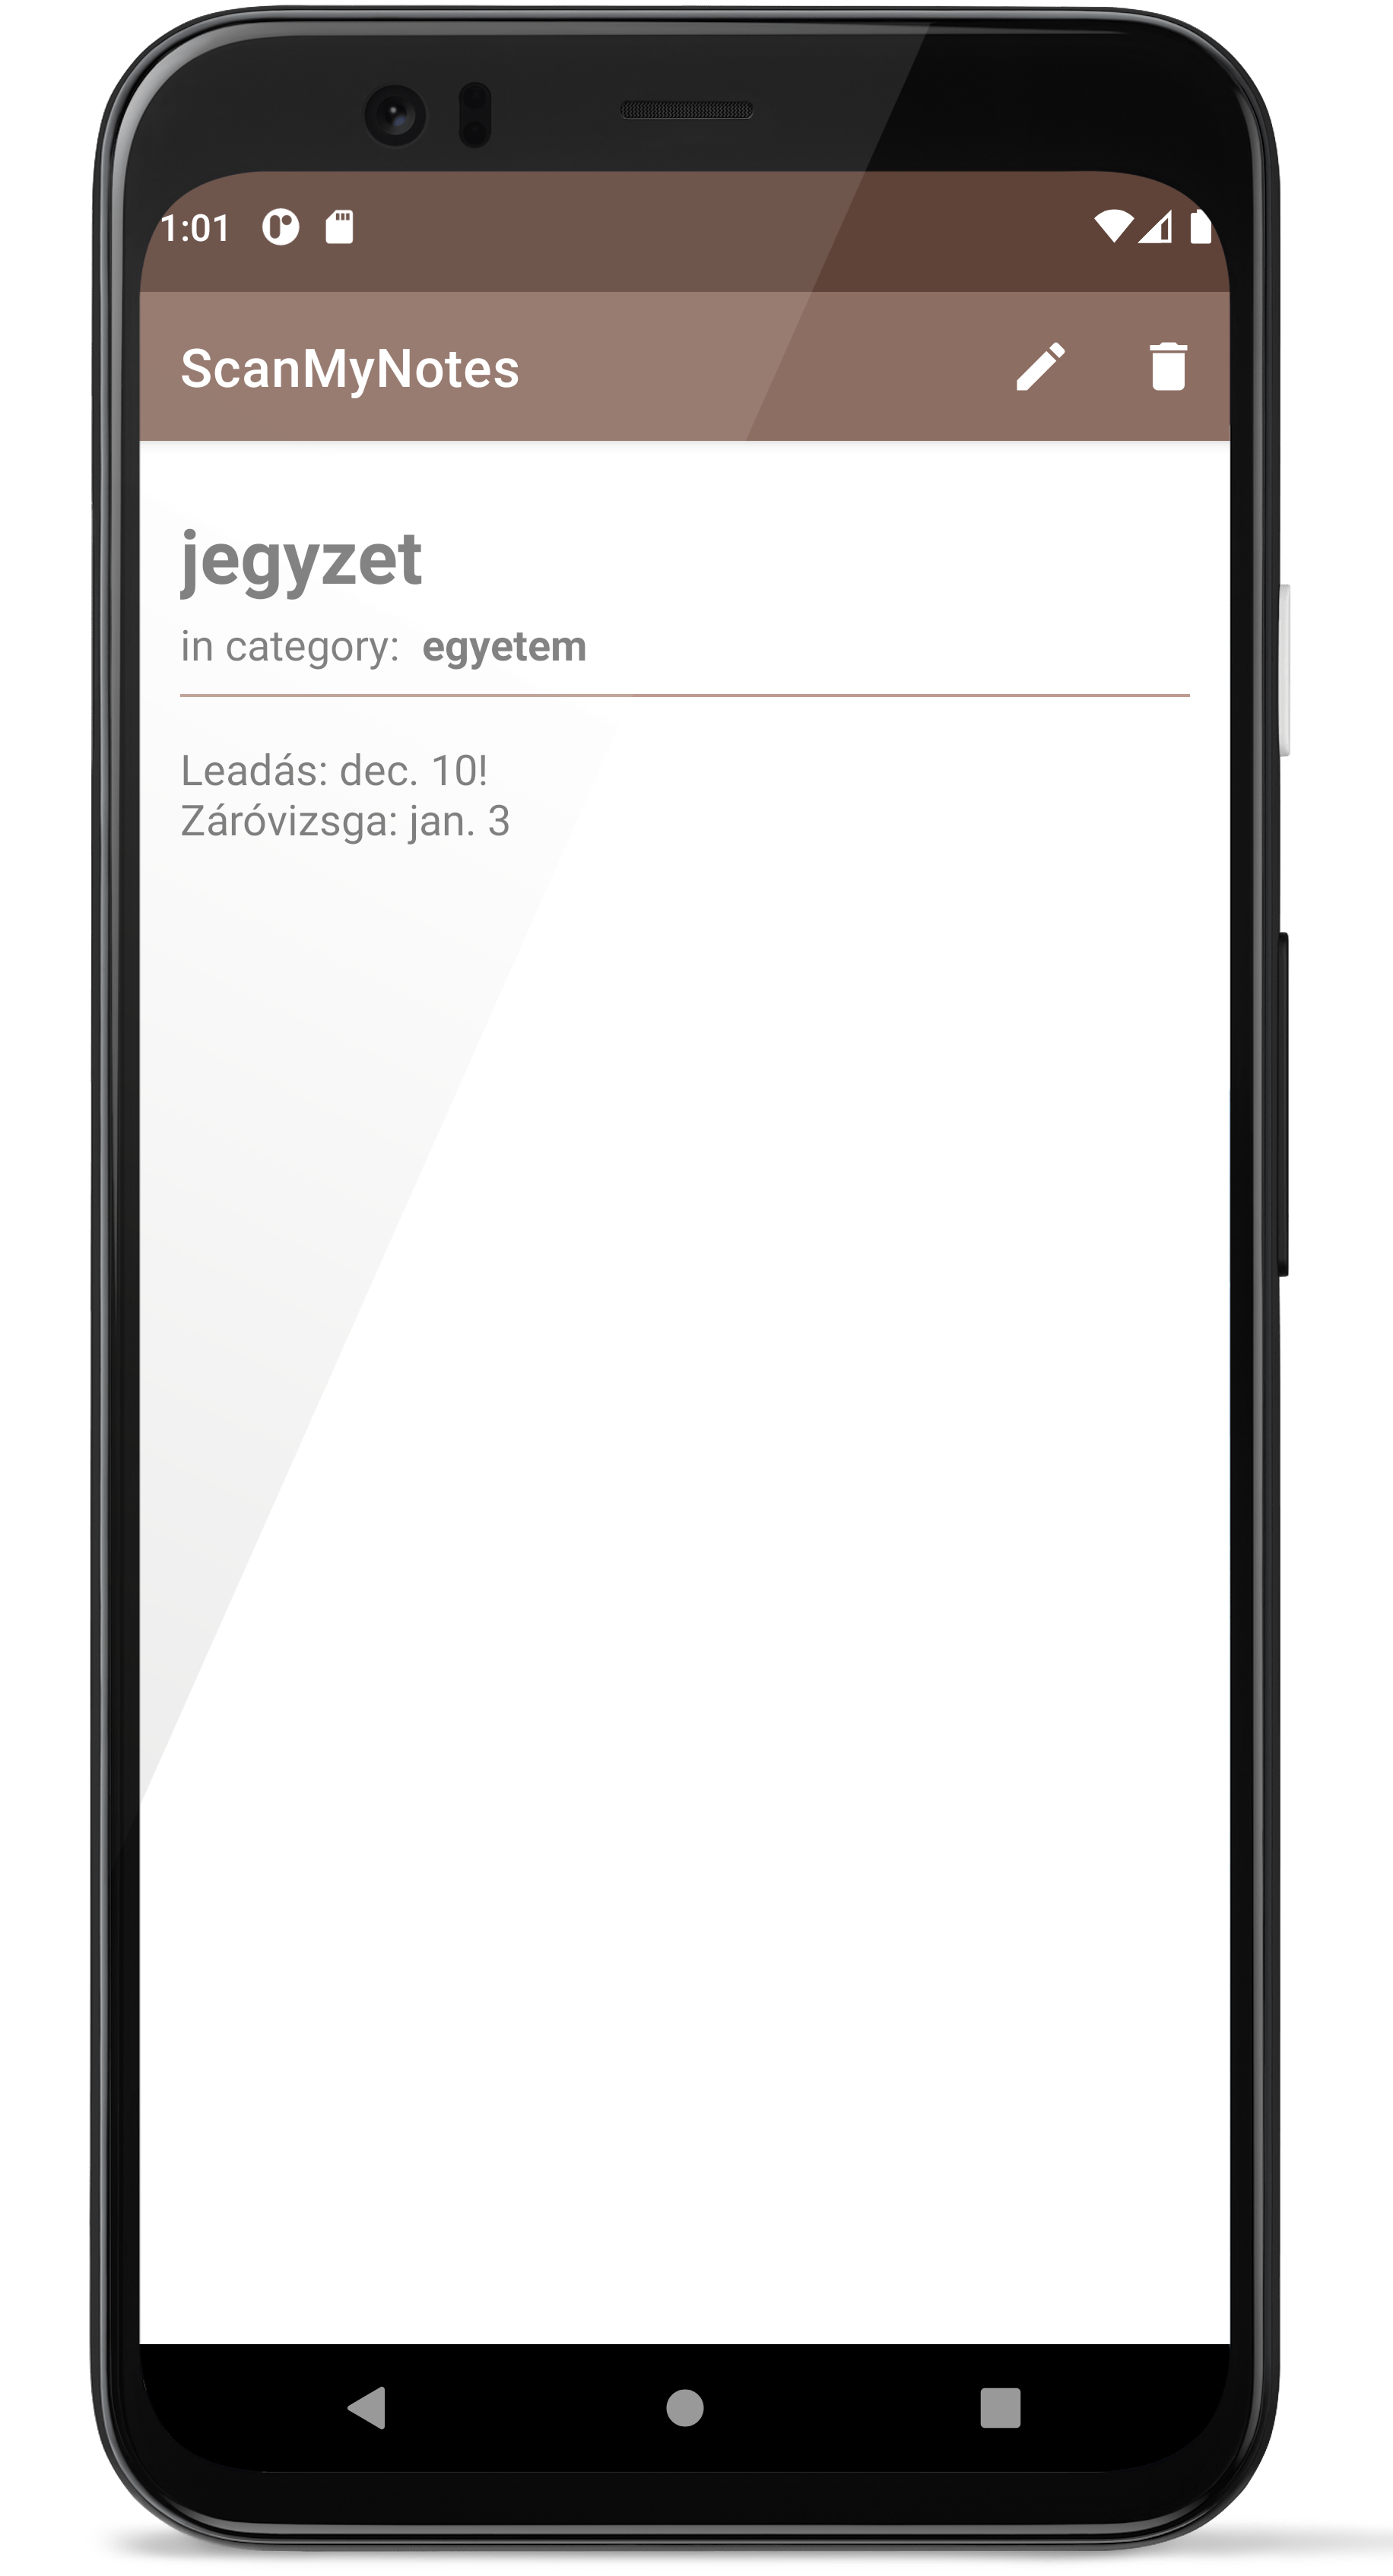
\includegraphics[width=55mm, keepaspectratio]{figures/note_view.png}
	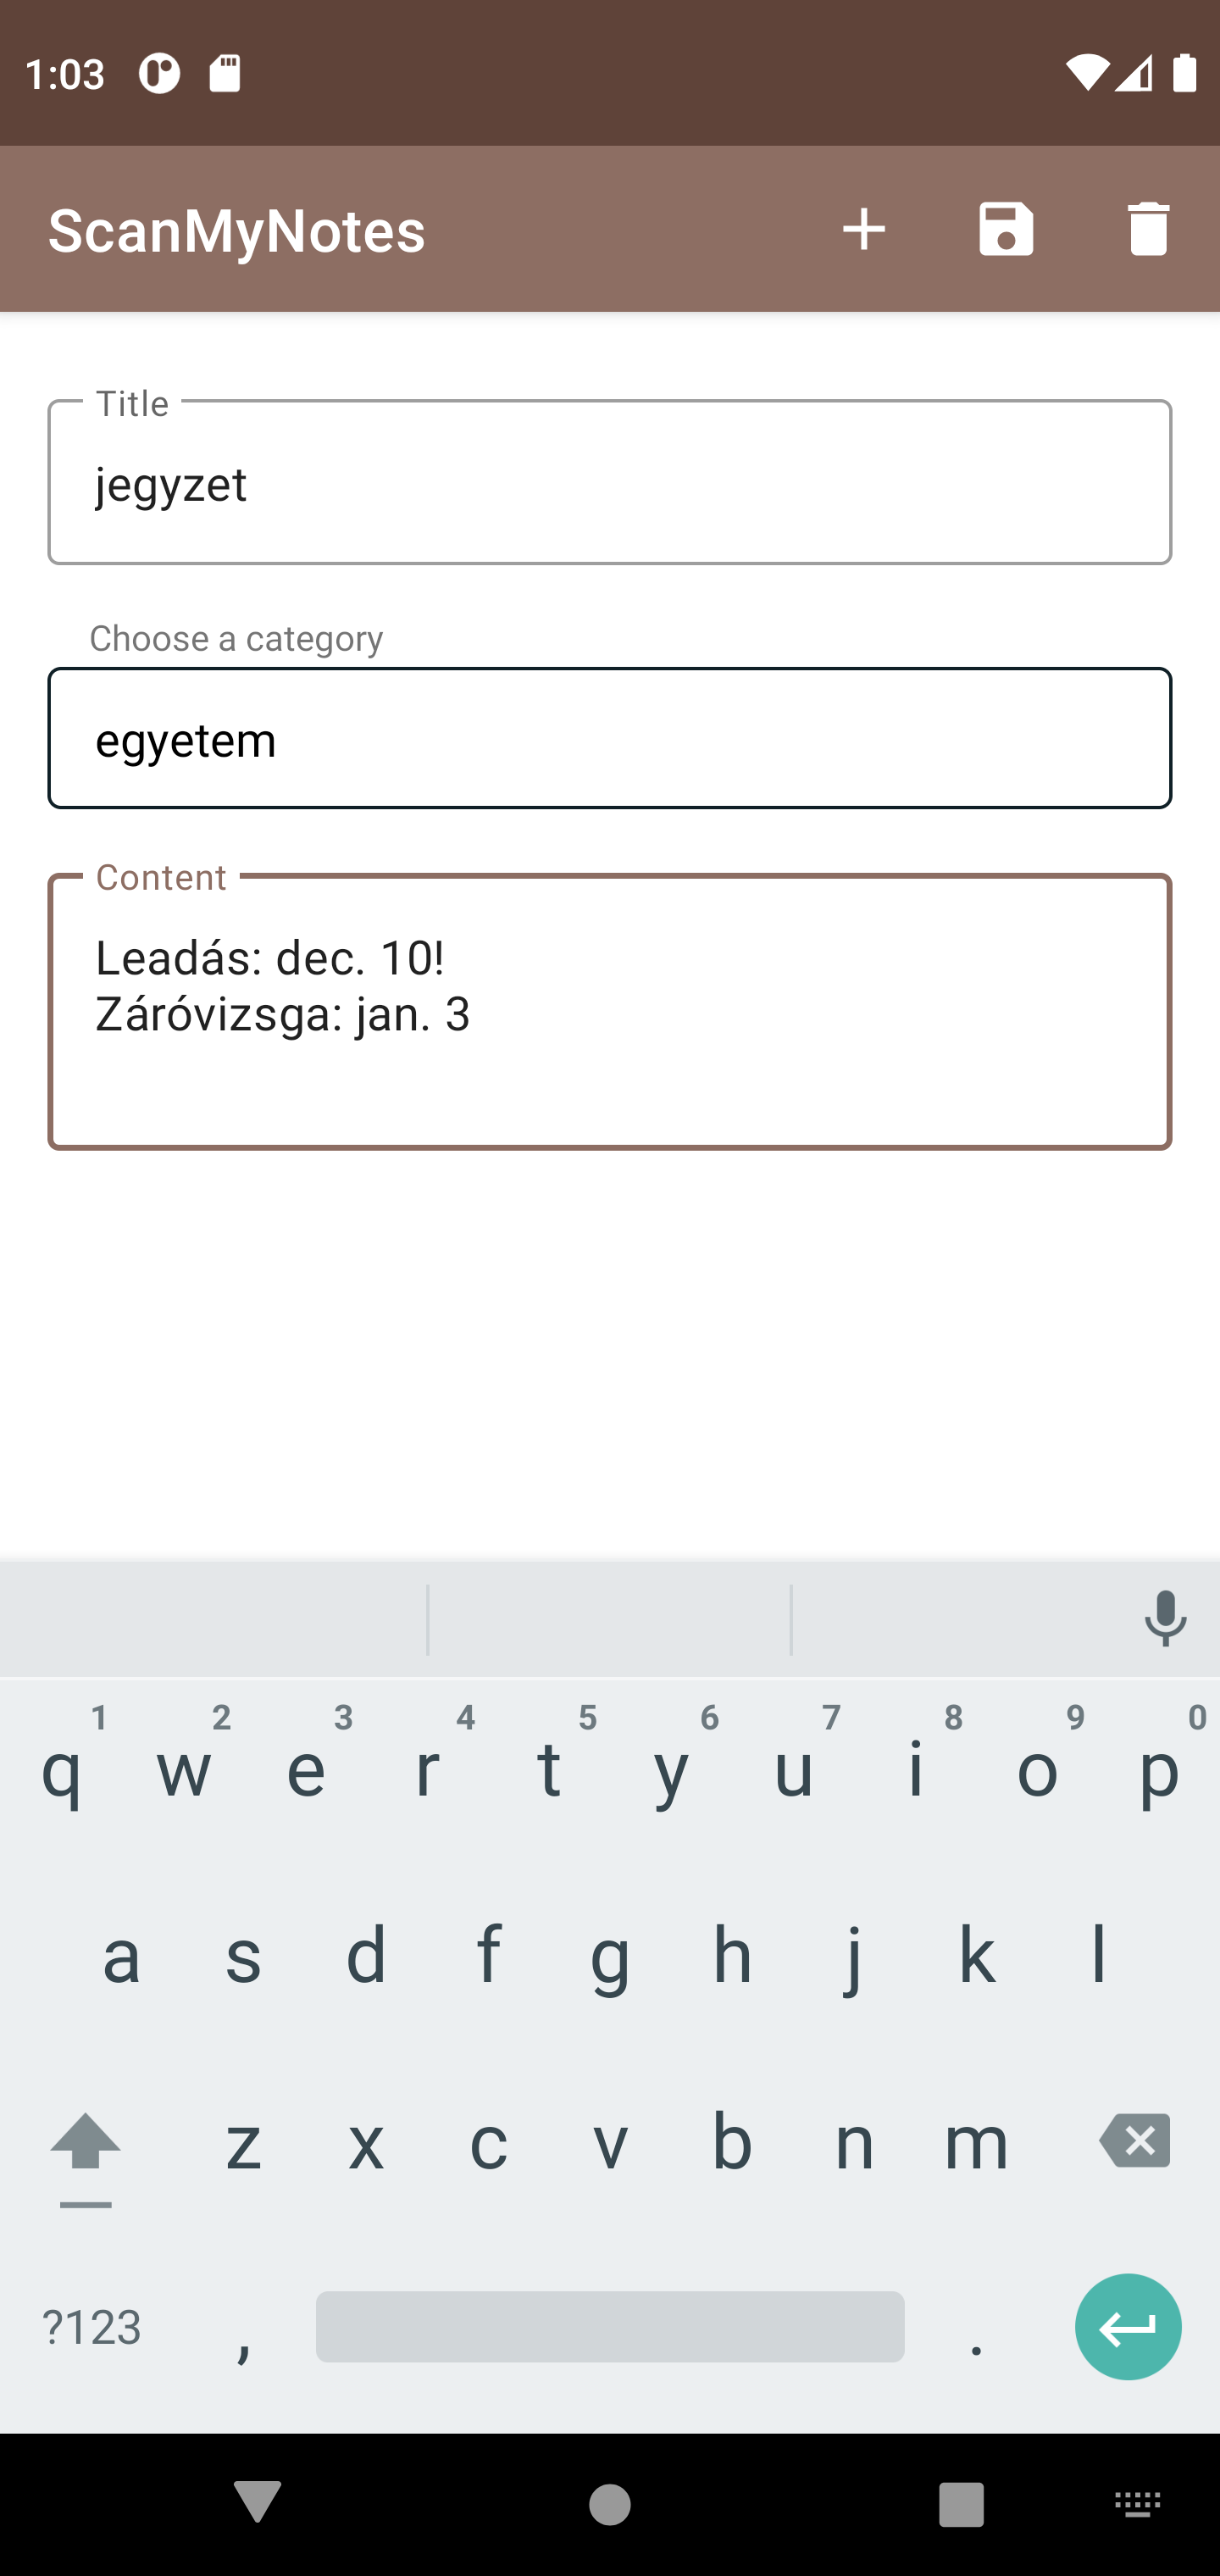
\includegraphics[width=55mm, keepaspectratio]{figures/note_edit.png}
	\caption{A jegyzet megtekintési, illetve szerkesztési képernyője.}
	\label{fig:NoteDetailsScreen}
\end{figure}

\subsection{Kategória létrehozása}
Az alkalmazásban elérhető másik adattípus a kategória, mely rendszerezési célt szolgál. Képes magába foglalni jegyzeteket és más kategóriákat is, tetszőleges mélységben. Szintén a jobb alsó sarokban található gomb biztosítja a létrehozás lehetőségét, ám ebben az esetben a felugró két kisebb gomb közül a felsőt kell választani. Itt egy, a jegyzetkészítéshez nagyon hasonló oldalon tudunk címet és opcionálisan szülőkategóriát megadni, és amennyiben nem üres a cím mezője, el is menthetjük (\refstruc{fig:NewCategoryScreen}). 

\begin{figure}[!ht]
	\centering
	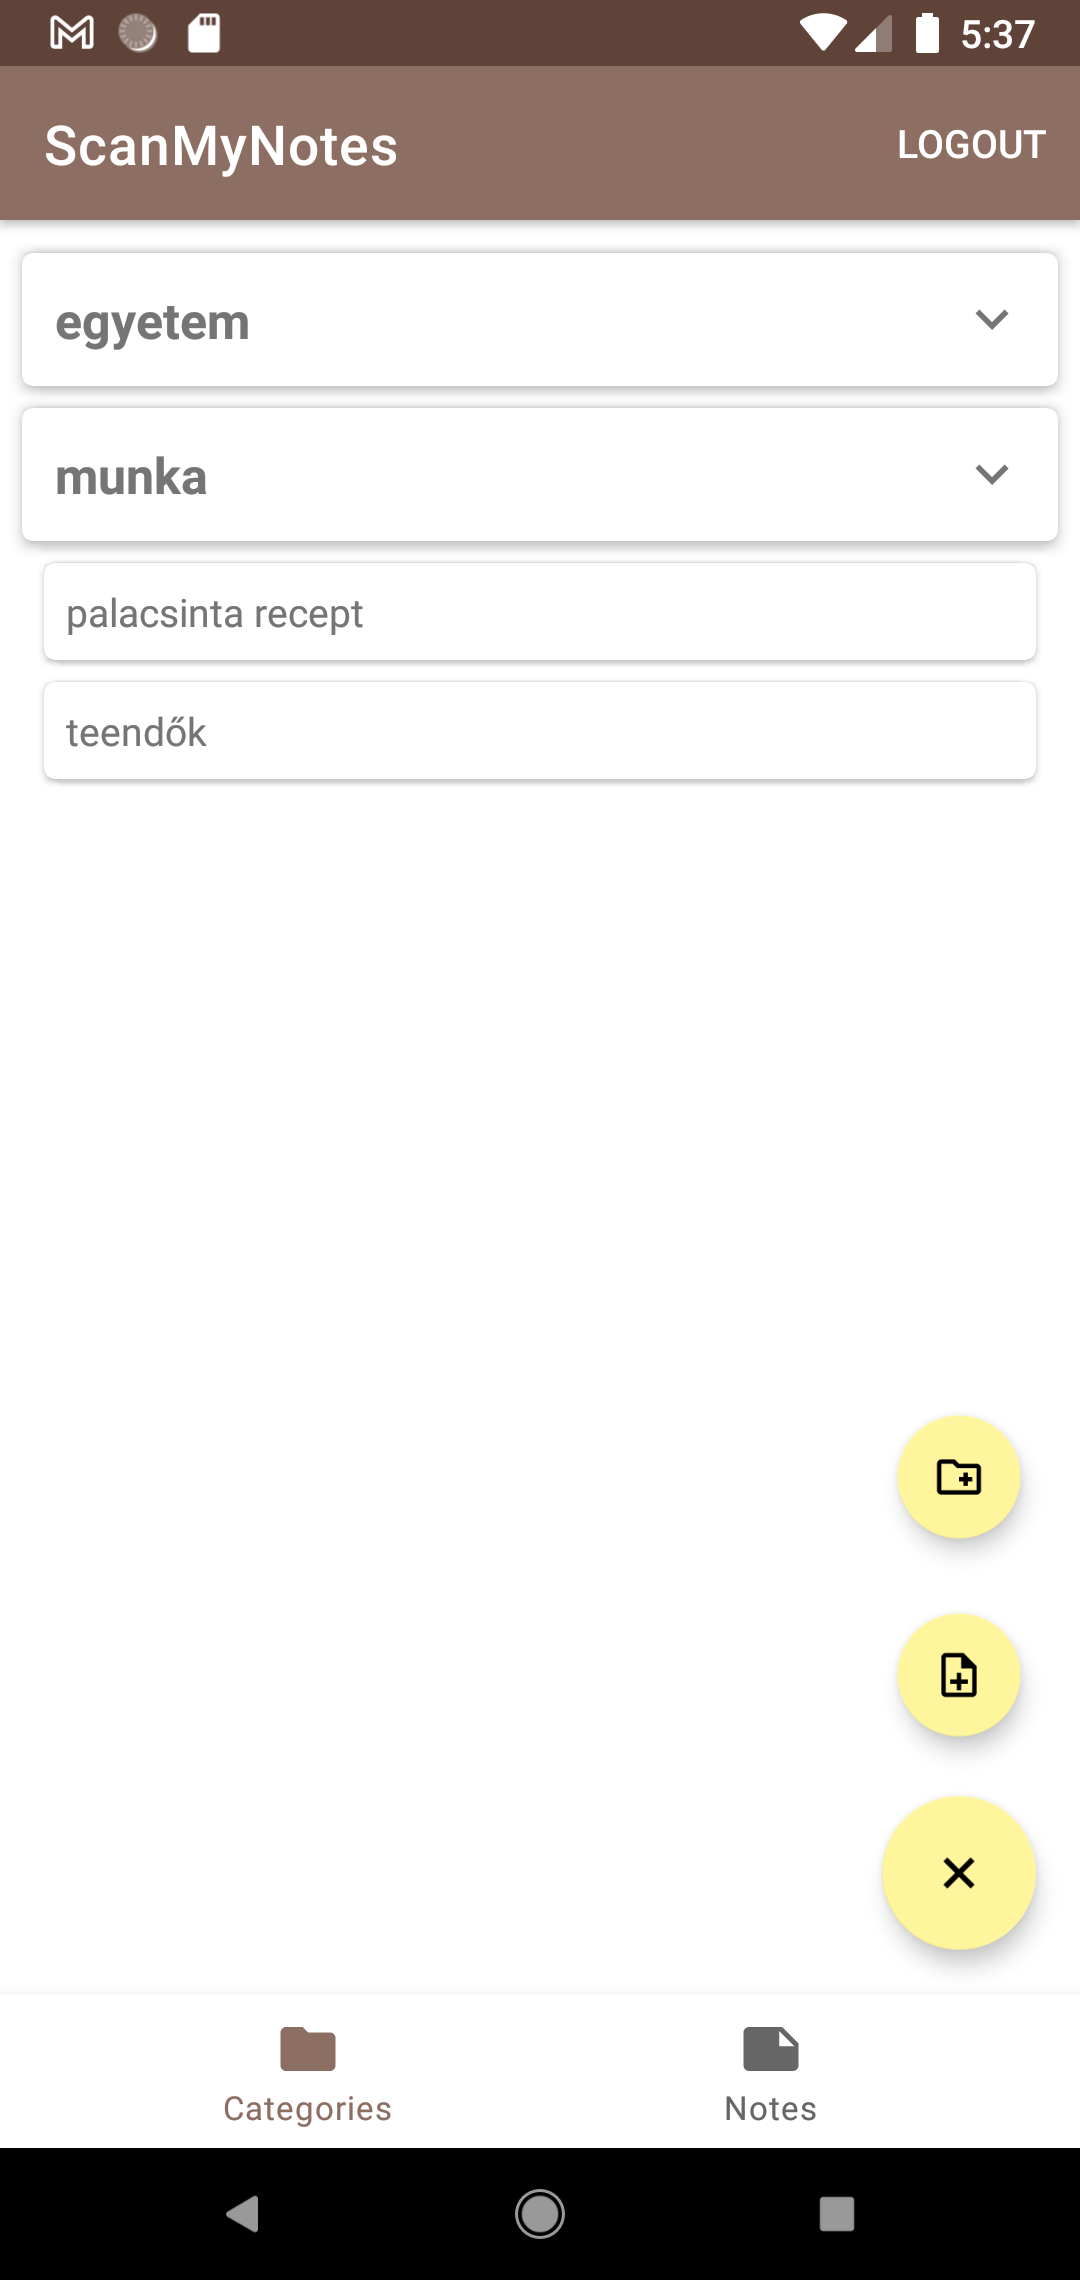
\includegraphics[width=50mm, keepaspectratio]{figures/floatingbutton_open.png}
	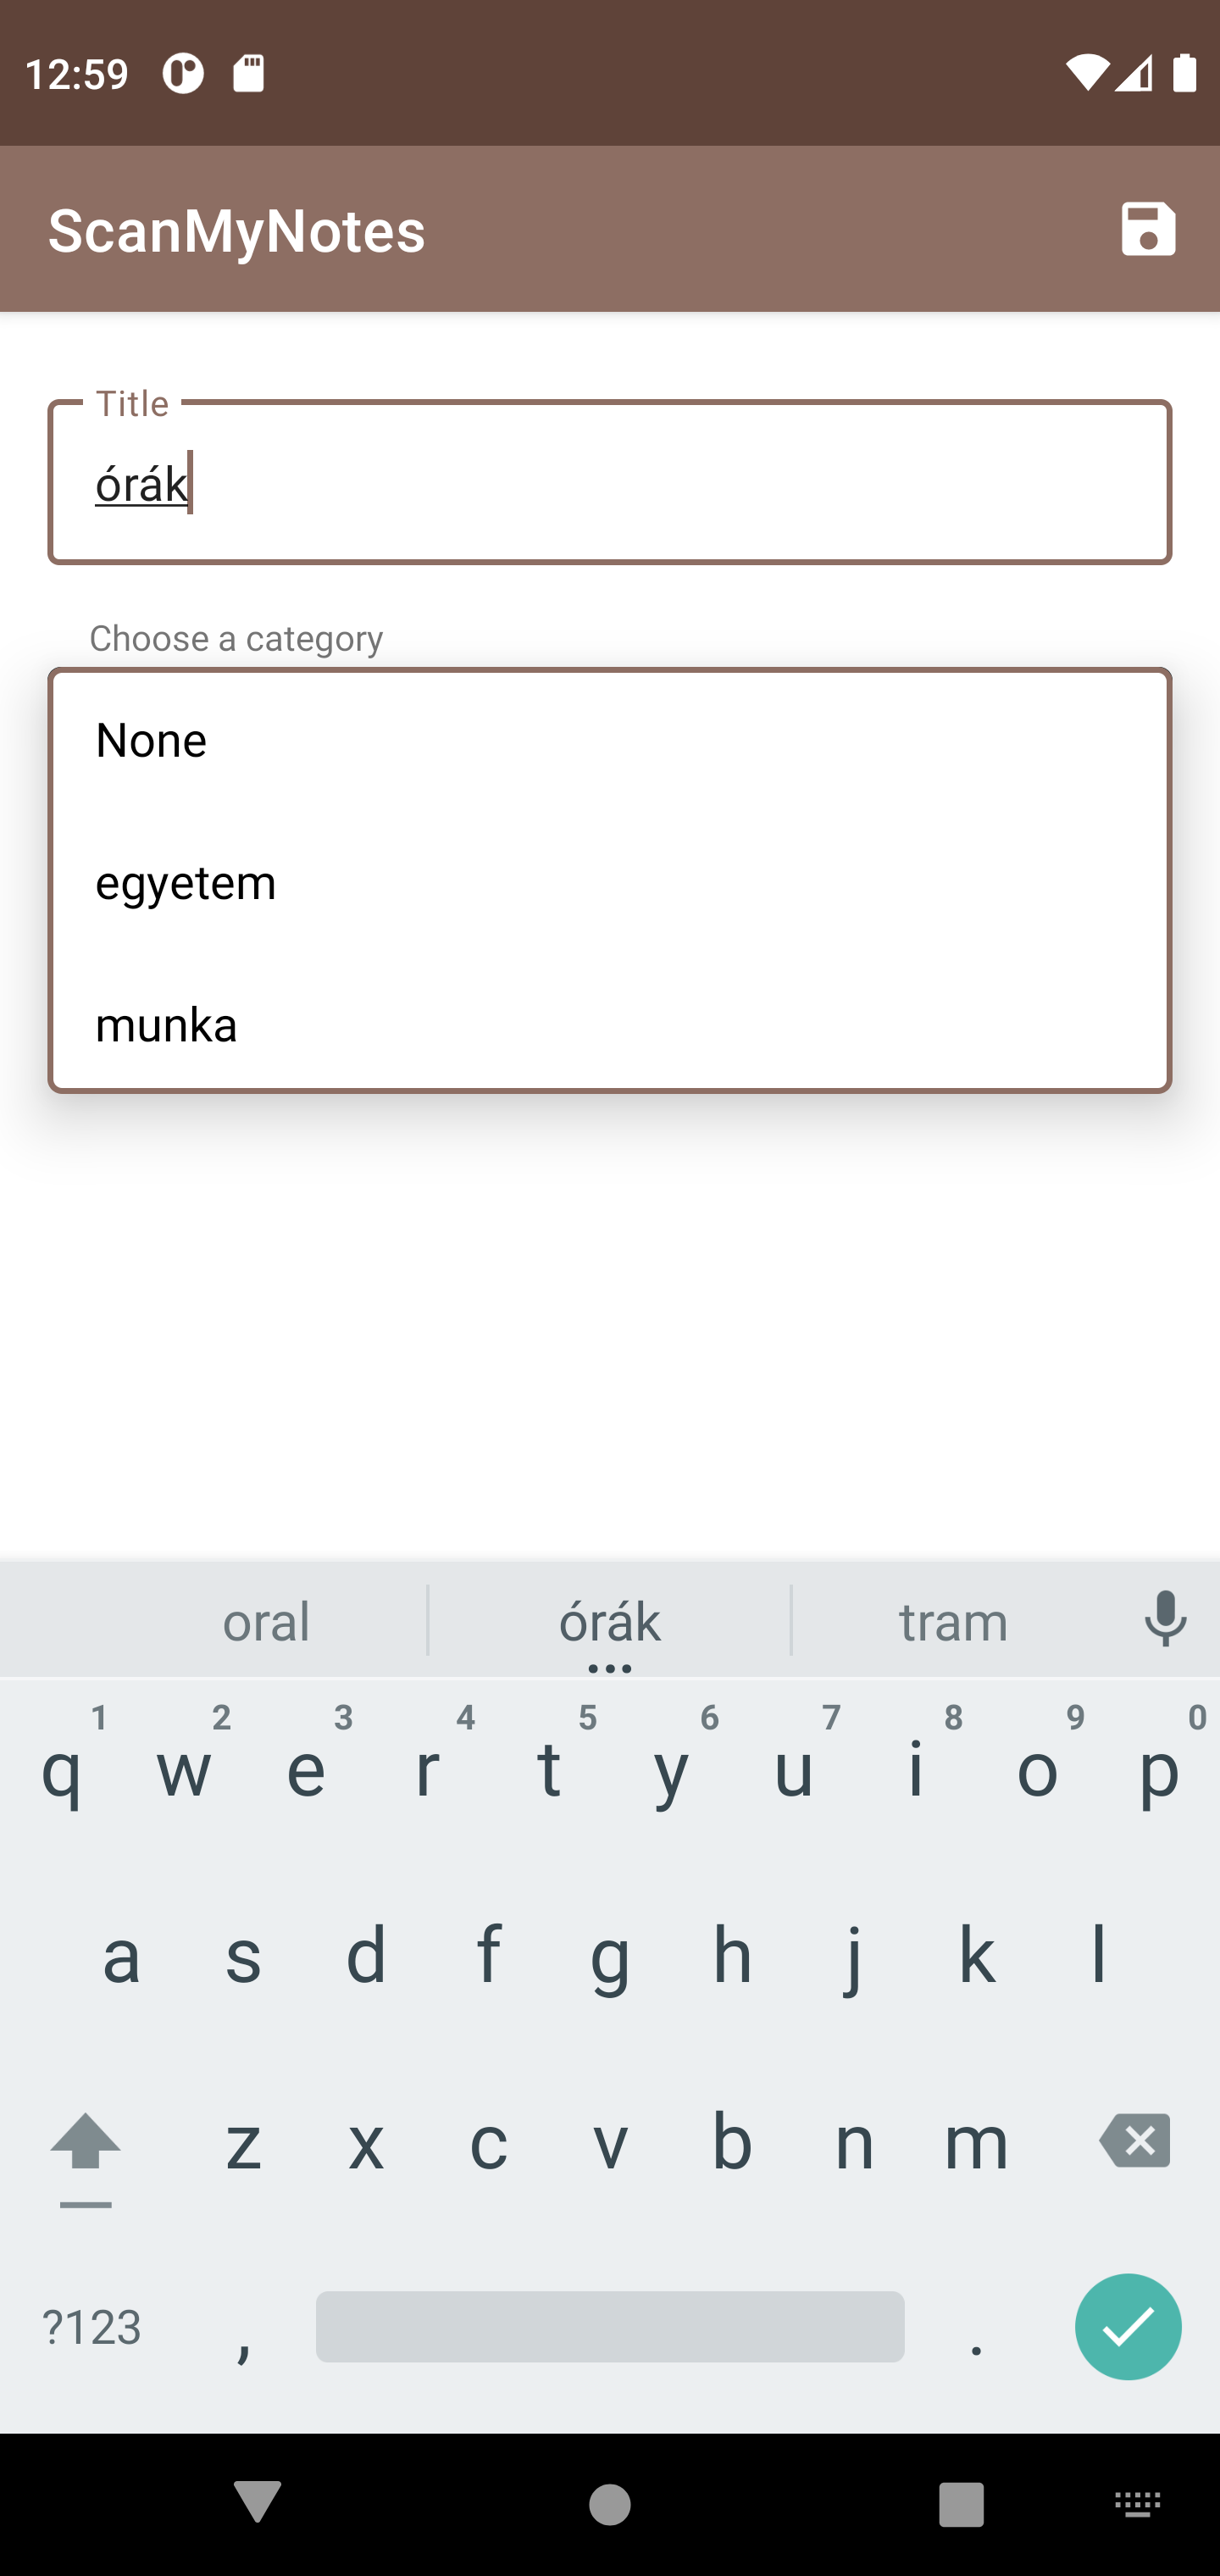
\includegraphics[width=50mm, keepaspectratio]{figures/category_save.png}
	\caption{A létrehozás gomb kinyitott állapotban, új kategória felvétele.}
	\label{fig:NewCategoryScreen}
\end{figure}

\subsection{Kategória szerkesztése}
Új kategória létrehozása után, illetve a listában egy kategóriára nyomva annak részleteit tekinthetjük meg. Itt megjelenik a címe és esetleges szülője, és jobb fent szintén található egy ceruza ikon, mely lehetővé teszi a szerkesztést (\refstruc{fig:CategoryDetailsScreen}). Hasonlóan a jegyzethez megtekintés és szerkesztés során is törölhetjük az adott kategóriát, ilyenkor egy felugró ablak figyelmeztet rá, hogy a törlés során az összes tartalmazott objektum is törlődni fog. 

\begin{figure}[!ht]
	\centering
	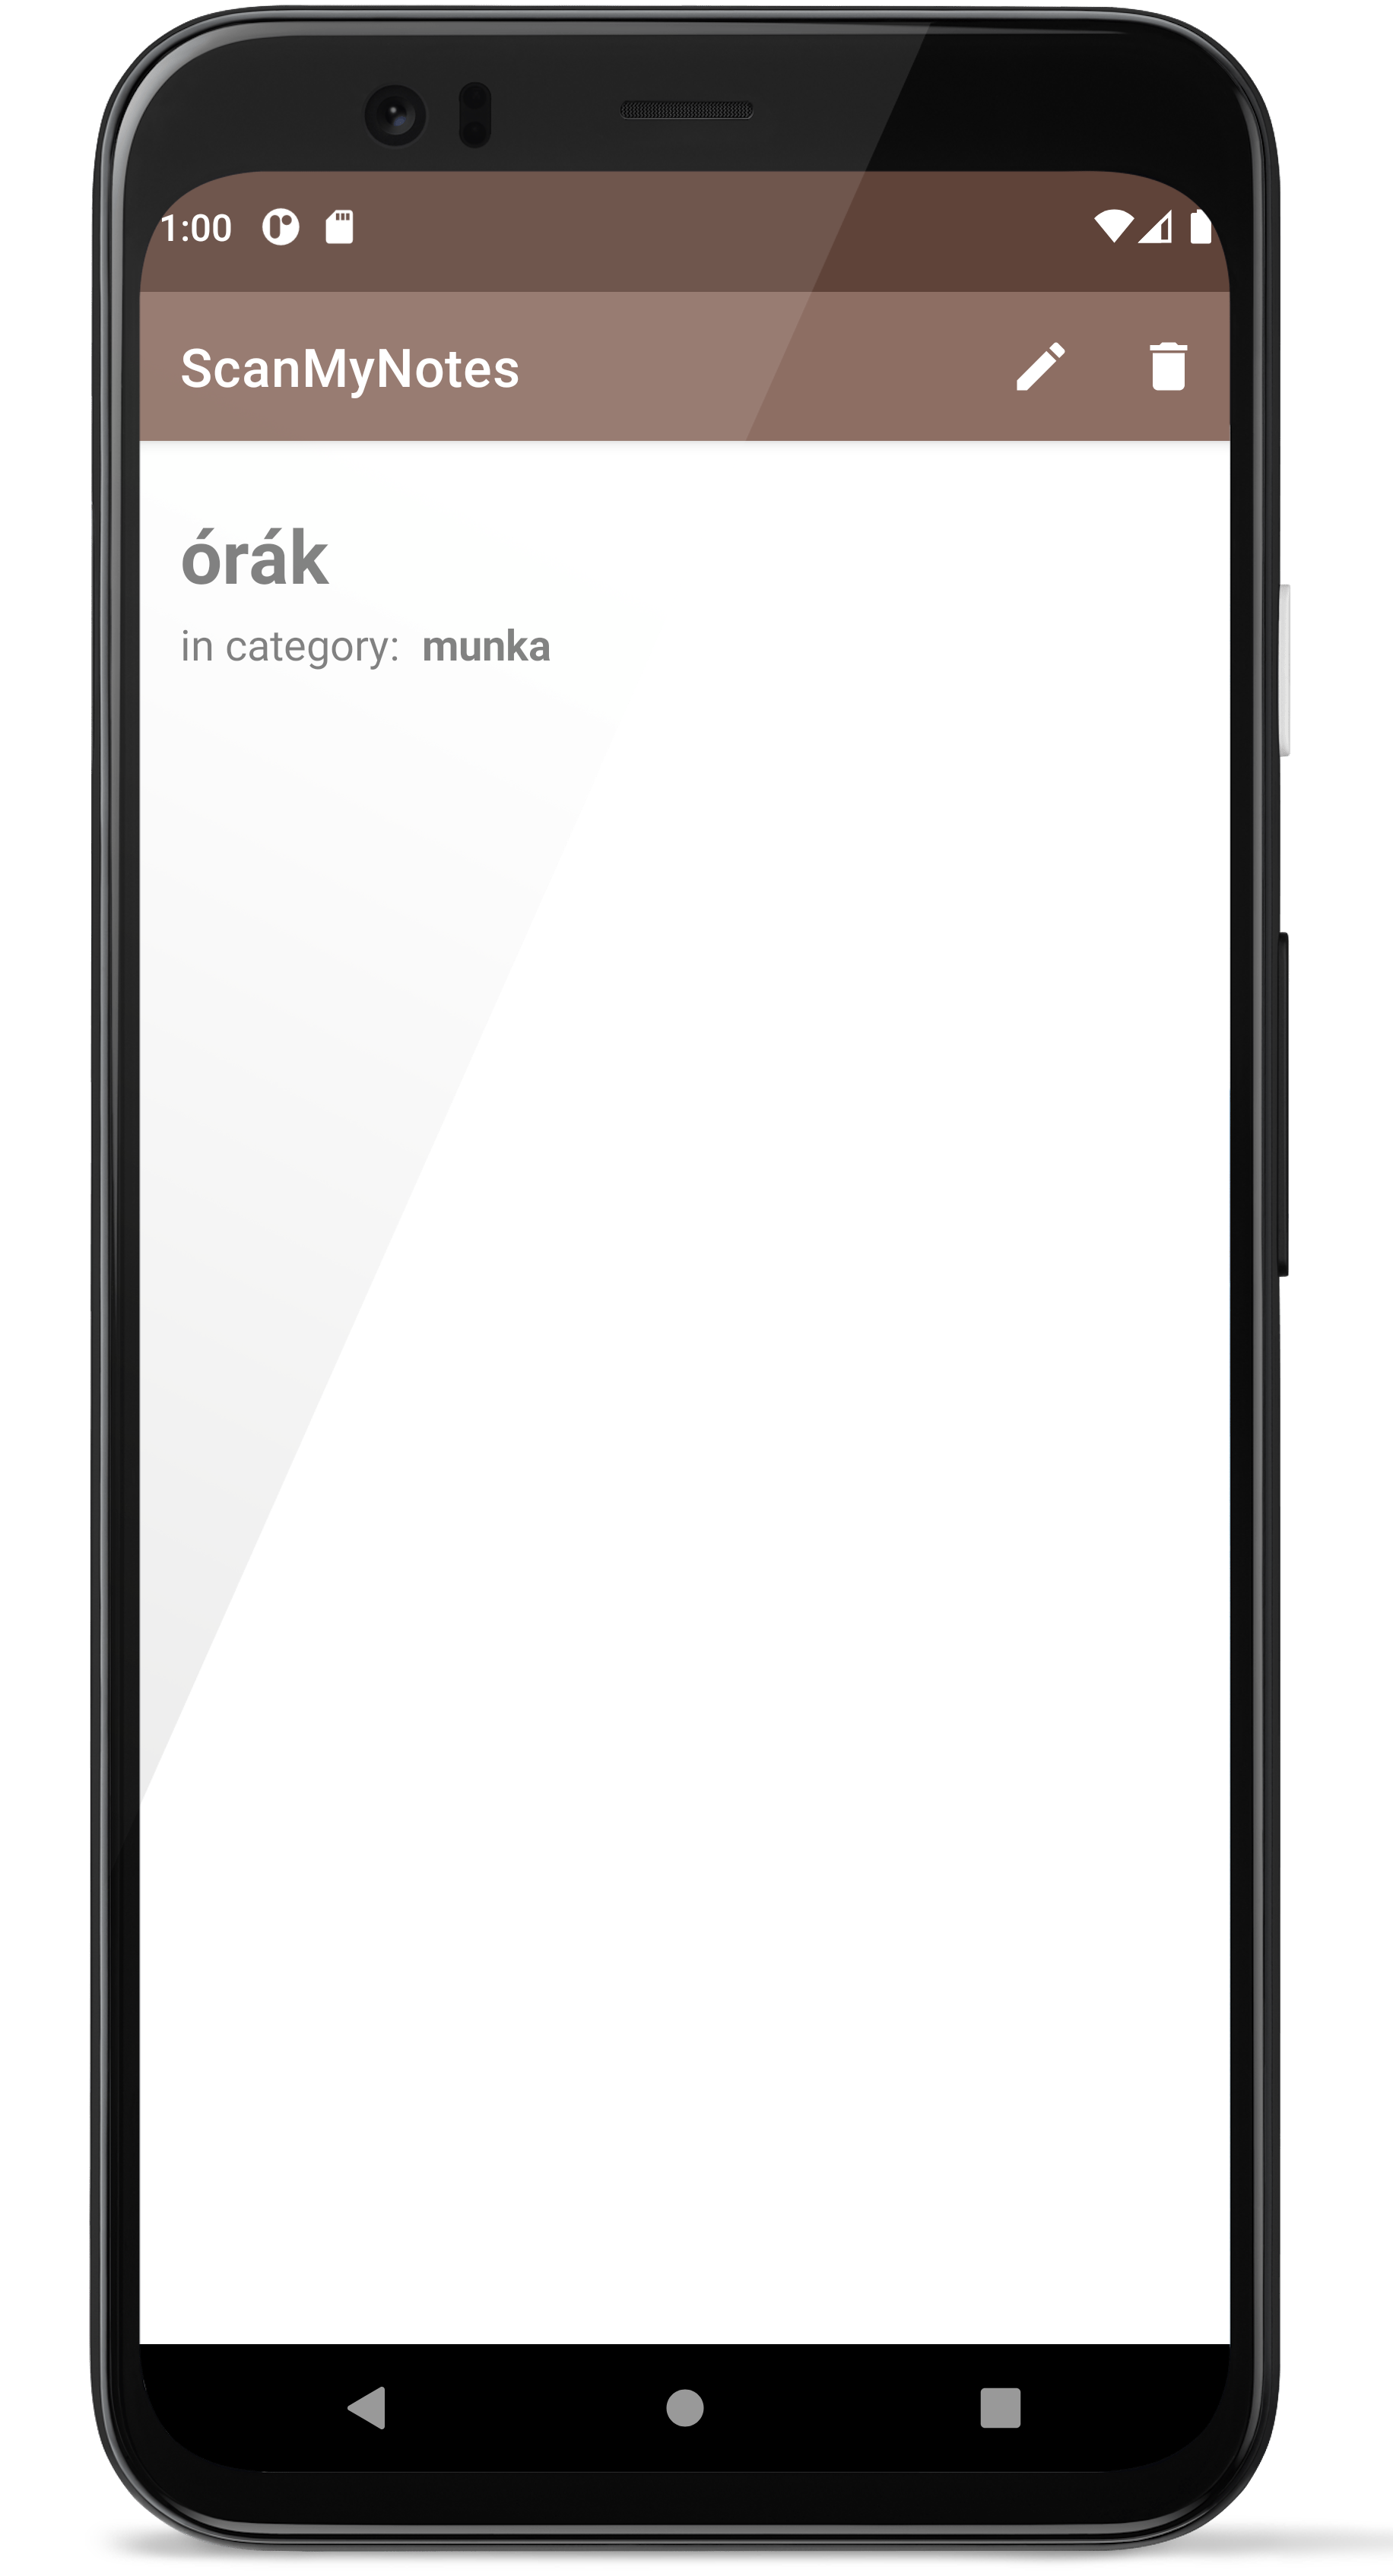
\includegraphics[width=50mm, keepaspectratio]{figures/category_view.png}
	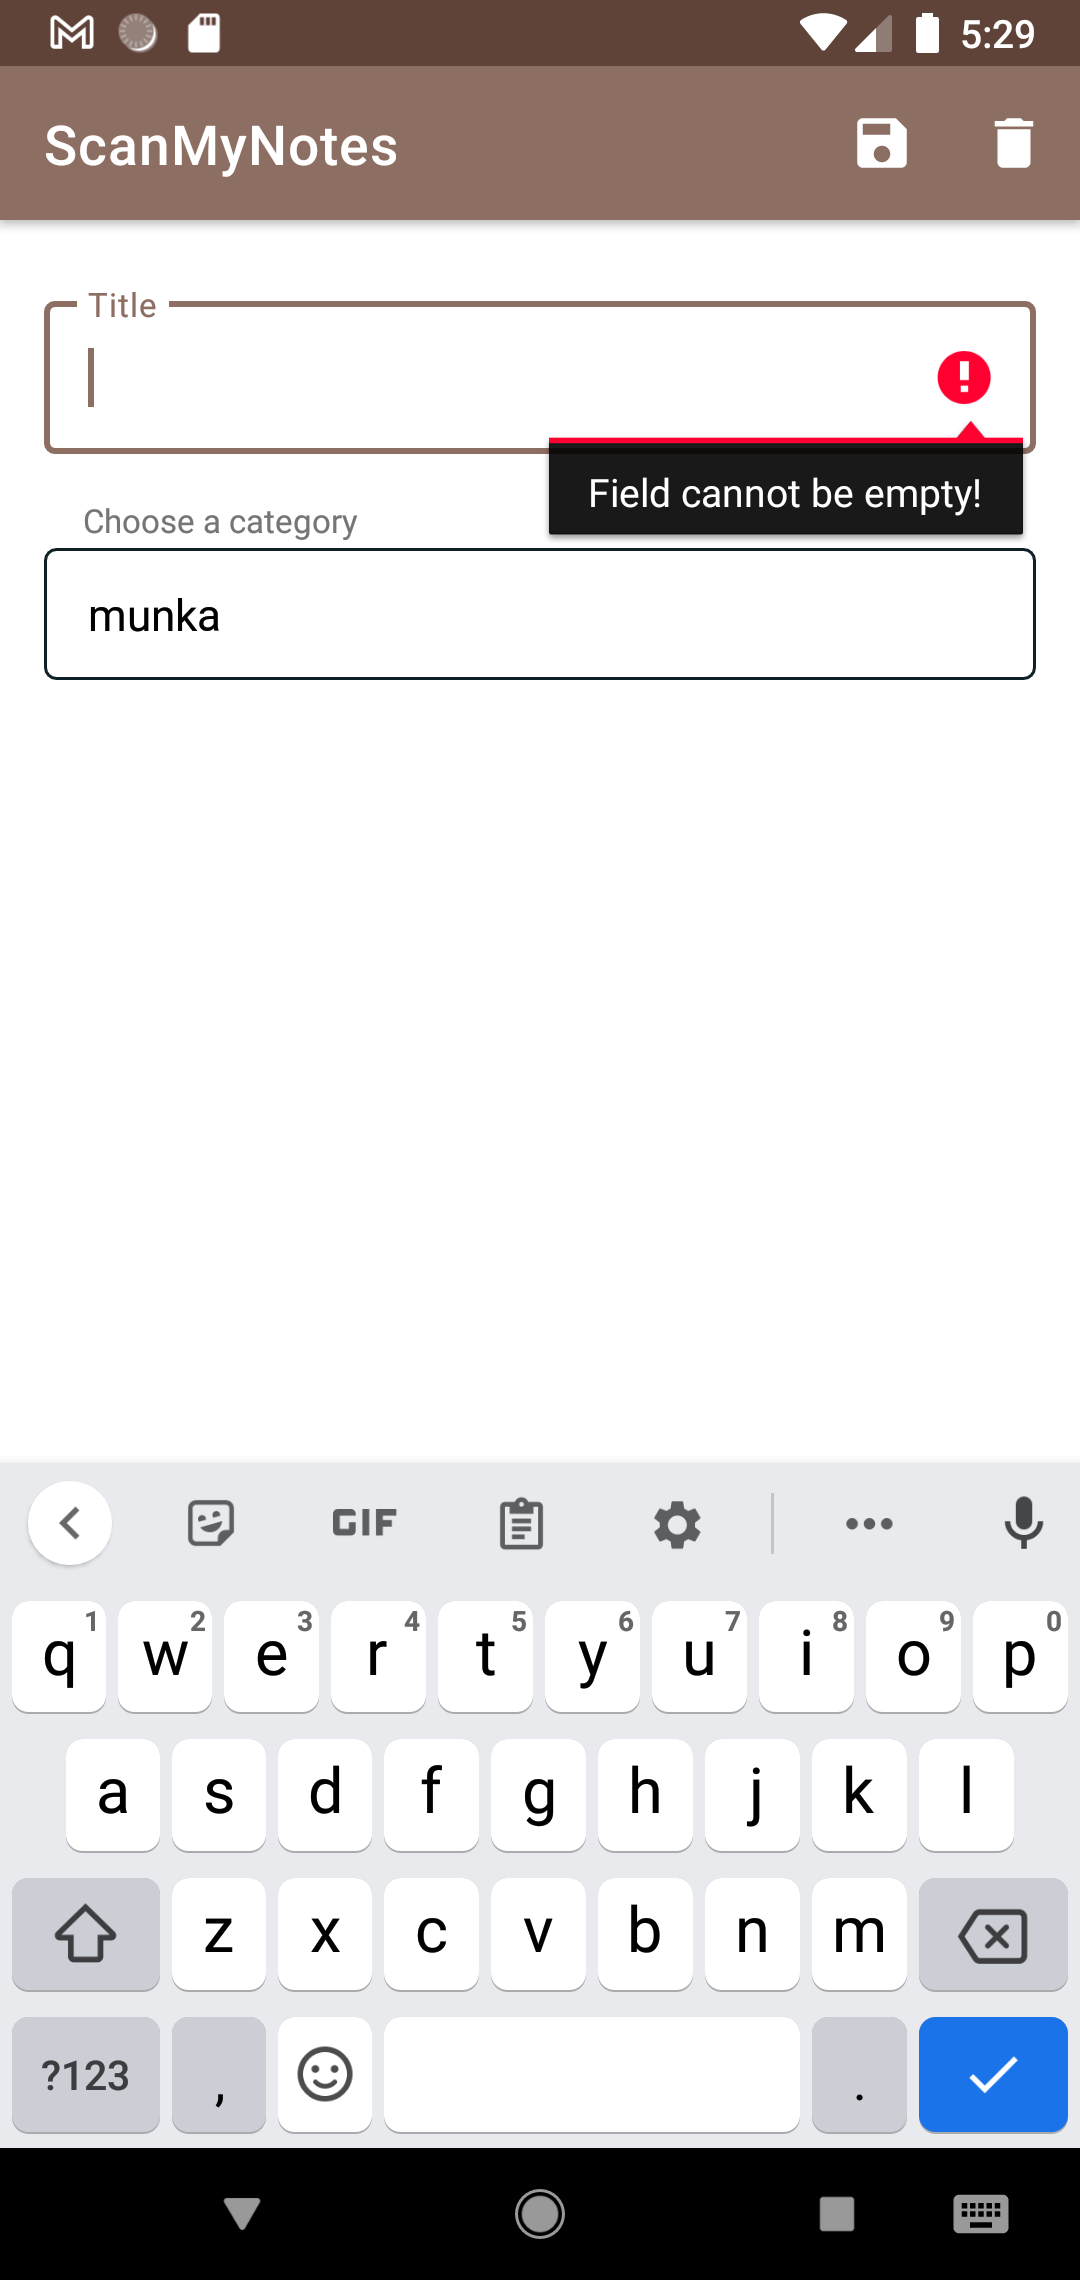
\includegraphics[width=50mm, keepaspectratio]{figures/category_edit_error.png}
	\caption{A kategória részletes képernyője, illetve a szerkesztési képernyő által feldobott hiba, ha üresen hagyjuk a címet.}
	\label{fig:CategoryDetailsScreen}
\end{figure}

\section{Tesztelés}